\documentclass{article}

\usepackage[a4paper]{geometry}

\usepackage{amsmath}
\usepackage{amssymb}
\usepackage{amsthm}
\usepackage{amsfonts}
%llbracket and rrbracket
\usepackage{stmaryrd}

\usepackage[boxed,noline]{algorithm2e}

\usepackage{float}
\usepackage{tikz}

\usetikzlibrary{automata}

%Defs and thms
\theoremstyle{definition}
\newtheorem{defi}{Definition}
\newtheorem{ex}[defi]{Example}

\theoremstyle{remark}
\newtheorem{rem}[defi]{Remark}

\theoremstyle{plain}
\newtheorem{thm}[defi]{Theorem}
\newtheorem{prob}[defi]{Problem}
\newtheorem{cor}[defi]{Corollary}
\newtheorem{lem}[defi]{Lemma}

%operators
\newcommand{\val}{\operatorname{val}}
\newcommand{\until}{\ \mathcal{U}}

\tikzset{every node/.style={align=center}, >= latex, font=\scriptsize}

\newcommand{\comm}[1]{{\color{red} \marginpar{? [?]} \textsf{[#1]}}}


\title{Survey of Hybrid Automata and their Abstractions}
\author{Ruth Hoffmann}

\begin{document}
\maketitle


\begin{abstract}
With the wide applicability of hybrid systems in the real world, it is now more than ever important to be able to verify these systems for safety and reliability. This paper surveys a number of abstraction techniques which turn these continuous systems into discrete, which can be verified with a variation of tools.
\end{abstract}

\section{Introduction}
\label{sec:intro}
We model and analyse complex systems using a range of mathematical formalisms and techniques. The type of system dictates the formalism used. For example, a system exhibiting continuous behaviour (a system of chemical reactions, fluid flow, movement of an aircraft, say) can be modelled using a set of differential equations, whereas a discrete state system can be modelled as finite state transition systems (or Finite State Automata---FSAs), or as Markov chain variants. An extension to finite state automata including real-timed clocks---Timed Automata (TAs) are used to model systems with additional time-dependent behaviour, such as real time systems or networks.


Some systems exhibit both discrete and continuous behaviour and so can not be modelled as a FSA or a set of differential equations alone (for example mutual-exclusion protocols \cite{Alur1995a}, temperature regulation \cite{Nicollin1993,Amin2006,Raskin2005}, water level regulation \cite{Alur1993}, train controllers \cite{Platzer2011a}, aircraft landing \cite{Tomlin2003}, robot cooperation \cite{Chaimowicz2003} and robotic decision making \cite{Dennis2013}).
These systems are known as hybrid systems and can be modelled using hybrid automata (HAs)---where continuous behaviour is modelled using differential equations within a finite set of {\it locations} (or {\it modes}) and discrete behaviour as discrete transitions between the modes. Being able to verify a hybrid system is crucial to show that the modelled real world application is safe \cite{Livadas1998a,Prajna2007}. However, unlike FSAs, which can (at least theoretically) be analysed using explicit or symbolic search of the statespace, HAs --- thanks to their continuous component---can not (although the state reachability problem for TAs, which are a special class of HAs is decidable \cite{Alur1994}).
There are various techniques on how to build a verifiable representation of a HA, as well as numerous tools. This paper focuses on abstraction techniques, which yield a finite system, or a system that can be verified using current model checking approaches. The abstractions do not use common notation, and some are special cases. We unify these.

Other systems, in addition to continuous and discrete behaviour, have probabilistic (stochastic) attributes, and can be modelled using stochastic hybrid automata (SHAs). When this stochastic behaviour translates as probabilistic transitions between locations, the automata are known as Probabilistic Hybrid Automata (PHAs). Otherwise, the stochastic behaviour is within the locations themselves (and represented as a set of distributions).
Like HAs, the verification of SHAs requires abstraction to a simpler, verifiable form, often using techniques similar to those used for their non-stochastic counterparts.

In this paper, we survey HAs and SHAs and their abstractions. We first introduce HAs and SHAs (Sections~\ref{sec:hybrid} and \ref{sec:stoch} respectively). In Section~\ref{sec:background} we provide some additional relevant background material and in
Sections~\ref{sec:abs} and \ref{sec:propabs} we present the different abstraction techniques of HAs and PHAs respectively, and a translation of SHAs to PHAs. %Finally, in Section~\ref{sec:related} we present relevant additional related work and tools. \comm{May not need last section?}


\section{Hybrid Automata}
\label{sec:hybrid}
The formal definitions of hybrid systems vary slightly, but they all agree on the following. A hybrid system consists of continuous and discrete variables. It is represented by finite state automata, where each mode (or location) of the automaton contains continuous actions, and the transitions between modes are discrete actions. The transitions are triggered through predicates defined on the continuous or discrete variables. This representation of a hybrid system is called a hybrid automaton.

\begin{defi}[Hybrid Automaton]
A \emph{hybrid automaton} $\mathcal{A}=(V,L,A,Init,Inv,E,f)$ consists of 7 components;
\begin{description}
    \item[$V$]{Finite set of \emph{continuous variables}, with valuation $\val(V)\subseteq\mathbb{R}^n$ where $n=|V|$,}
    \item[$L$]{Finite set of \emph{locations/modes/discrete variables},}
    \item[$A$]{Finite set of \emph{actions},}
    \item[$Init$]{Set of \emph{initial states}, $Init\subseteq L \times \val(V)$,}
    \item[$Inv$]{\emph{Invariant condition}, $Inv: L \rightarrow 2^{\val(V)}$,}
    \item[$E$]{Finite set of \emph{edges}, $E\subseteq L\times A\times L$, where each edge represents a transition between two modes, and is labelled with an action and the following
        \begin{itemize}
            \item{$g : E \rightarrow 2^{\val(V)}$, a \emph{guard},}
            \item{$r : E \rightarrow 2^{\val(V)}$, a \emph{reset map},}
        \end{itemize}}
    \item[$f$]{\emph{Flow condition}, $f: L\rightarrow (\val(V)\rightarrow\val(V))$.}
\end{description}
\end{defi}

The set of states of the automaton is defined by $L\times\val(V)$. The invariant condition labels the modes with the domain of each continuous variable, while the flow function defines the behaviour of the continuous variables. For each mode $\ell\in L$ the flow of the continuous variable $x\in V$ is governed by the differential of $x$, $\dot{x}=f(\ell)(x)$.

The execution of a hybrid system, follows the semantics of the hybrid automaton, by using the set of states $L\times\val(V)$, starting in the initial states $Init$ and following two types of transitions. Firstly, the discrete transitions, which correspond to the edges $e\in E$ in the hybrid automata definition and secondly, the continuous transitions which correspond to the flow condition.

\begin{rem}[\cite{Halbwachs1994}]
The edges of the underlying automaton can be seen as transition functions, and through their reset map can change the current valuation of a continuous variable.
\end{rem}

\begin{ex}[Thermostat \cite{Henzinger2000}]
We take a simple example to illustrate a hybrid system and its corresponding automaton. Assume we have a thermostat controlling the temperature of a room. If the temperature falls beneath a certain limit, we turn the heating on, until it reaches a certain temperature. Once the upper temperature limit is reached, we turn the heating off, and so on. The automaton consists of the following $V=\{x\}$, $val(V)\subseteq\mathbb{R}$, $L=\{l_{0},l_{1}\}$, $A=\{ON,OFF\}$ and $Init=(l_{0},x\geq18)$. Each mode is labelled with the invariant condition
\begin{align*}
    Inv(l_{0}) & = \{x\geq18\} \\
    Inv(l_{1}) & = \{x\leq22\}
\end{align*}
and the flow
\begin{align*}
    f(l_{0}) & = \{\dot{x} = -0.1x\} \\
    f(l_{1}) & = \{\dot{x} = 5-0.1x\}.
\end{align*}
Finally, the edges between the modes have got guards
\begin{align*}
    g(l_{0},ON,l_{1}) & = \{x<19\}  \\
    g(l_{1},OFF,l_{0}) & = \{x>21\}
\end{align*}
and the reset maps are empty.
Figure~\ref{fig:exthermo} shows the hybrid automaton of this example, with the labelled modes and transitions.
\begin{figure}[H]
    \begin{center}
        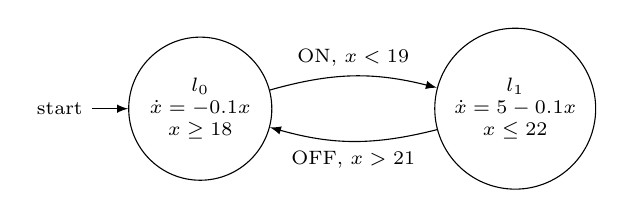
\begin{tikzpicture}[node distance=4cm]
            \node [state,initial] (s0) {$l_{0}$ \\ $\dot{x}=-0.1x$ \\ $x\geq18$};
            \node [state] (s1) [right of = s0] {$l_{1}$\\ $\dot{x}=5-0.1x$ \\ $x\leq22$};
            \path[->] (s0) edge [bend left=15] node [above] {ON, $x<19$} (s1)
                (s1) edge [bend left=15] node [below] {OFF, $x>21$} (s0);
        \end{tikzpicture}
        \caption{Hybrid Automaton of a thermostat.}
        \label{fig:exthermo}
    \end{center}
\end{figure}
\end{ex}

There are numerous types of hybrid systems which are defined by restrictions on their flow, guard and reset maps. In the next sections we are going to introduce the most common types.


%%%%%%%%%%%%%%%%%%%%%%%%%%%%%%%%%%%%%%%%%%%%%%%%%%%%%%%%%%%%%%%%%%%%%%%%%%%%%%%%%%%%%%%%%%%%%%%%%%%
%%%%%%%%%%%%%%%%%%%%%%%%%%%%%%%%%%%%%%%%%%%%%%%%%%%%%%%%%%%%%%%%%%%%%%%%%%%%%%%%%%%%%%%%%%%%%%%%%%%
%%% RECTANGULAR HA
%%%%%%%%%%%%%%%%%%%%%%%%%%%%%%%%%%%%%%%%%%%%%%%%%%%%%%%%%%%%%%%%%%%%%%%%%%%%%%%%%%%%%%%%%%%%%%%%%%%
%%%%%%%%%%%%%%%%%%%%%%%%%%%%%%%%%%%%%%%%%%%%%%%%%%%%%%%%%%%%%%%%%%%%%%%%%%%%%%%%%%%%%%%%%%%%%%%%%%%
\subsection{Rectangular Hybrid Automata}
A rectangular hybrid automaton constricts the behaviour of the continuous variables within the modes. The slope of the continuous variables in each mode can vary within a bounded or unbounded rational interval.
%\cite{Puri1994} \cite{Henzinger1995}

\begin{defi}[Rectangular Set]
For $\mathbb{R}^{n}$, with variables $x_{1},\ldots,x_{n}$, a \emph{rectangular set} is a conjuction of linear inequalities such as $x_{i}\sim c$, where $\sim\in\{<,\leq,=,\geq,>\}$, and $c\in\mathbb{Q}$. We say that for a rectangular set $R$, $R_{i}$ is the projection of $R$ onto $x_{i}$. So a rectangular set $R\subseteq\mathbb{R}^{n}$ is of the form $R=R_{1}\times\cdots\times R_{n}$.
\end{defi}

\begin{defi}[Rectangular Automaton]
A hybrid automaton $\mathcal{A} = (V,L,A,Init,Inv,E,f)$ is \emph{rectangular} if
\begin{itemize}
    \item{for every $\ell\in L$ the sets $Init(\ell)$ and $Inv(\ell)$ are rectangular,}
    \item{for every $\ell\in L$, there is a rectangular set $R^{\ell}$ such that $f(\ell)(x)=R^{\ell}$, $\forall x \in V$,}
    \item{and on every edge $e\in E$ the guard set $g(e)$, and reset map $r(e)$ are rectangular.}
\end{itemize}
\end{defi}

\begin{ex}[Rectangular Automaton Example \cite{Alur2000}]
Figure~\ref{fig:exrect} shows a generic example of a rectangular hybrid automaton. The slopes of the differential equations are within a given bound and all sets in the modes and on the edges are rectangular.
\begin{figure}[H]
    \begin{center}
        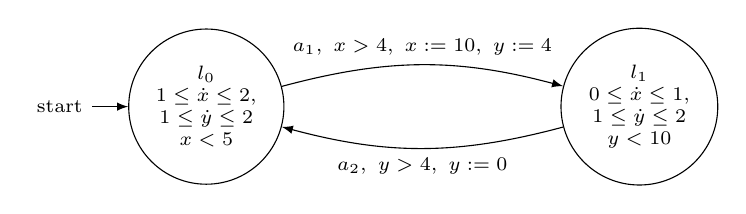
\begin{tikzpicture}[node distance=5.5cm]
            \node [state,initial] (s0) {$l_{0}$ \\ $1\leq\dot{x}\leq2,$\\$1\leq\dot{y}\leq2$ \\ $x<5$};
            \node [state] (s1) [right of = s0] {$l_{1}$ \\ $0\leq\dot{x}\leq1,$\\$1\leq\dot{y}\leq2$ \\ $y<10$};
            \path[->] (s0) edge [bend left=15] node [above] {$a_{1},\ x>4,\ x:=10,\ y:=4$} (s1)
                (s1) edge [bend left=15] node [below] {$a_{2},\ y>4,\ y:=0$} (s0);
        \end{tikzpicture}
        \caption{Example of a rectangular automaton.}
        \label{fig:exrect}
    \end{center}
\end{figure}
\end{ex}


%%%%%%%%%%%%%%%%%%%%%%%%%%%%%%%%%%%%%%%%%%%%%%%%%%%%%%%%%%%%%%%%%%%%%%%%%%%%%%%%%%%%%%%%%%%%%%%%%%%
%%%%%%%%%%%%%%%%%%%%%%%%%%%%%%%%%%%%%%%%%%%%%%%%%%%%%%%%%%%%%%%%%%%%%%%%%%%%%%%%%%%%%%%%%%%%%%%%%%%
%%% LINEAR HA
%%%%%%%%%%%%%%%%%%%%%%%%%%%%%%%%%%%%%%%%%%%%%%%%%%%%%%%%%%%%%%%%%%%%%%%%%%%%%%%%%%%%%%%%%%%%%%%%%%%
%%%%%%%%%%%%%%%%%%%%%%%%%%%%%%%%%%%%%%%%%%%%%%%%%%%%%%%%%%%%%%%%%%%%%%%%%%%%%%%%%%%%%%%%%%%%%%%%%%%
\subsection{Linear Hybrid Automata}
The characteristics of a linear hybrid automaton are the linear expressions of the continuous variables. \cite{Alur1995a} Linear automata are also called \emph{multirate automata} \cite{Alur1995a,Alur2000}.

\begin{defi}[Linear Term \cite{Henzinger2000}]
Let $k_{0},\ldots,k_{n}\in \mathbb{Z}$, and $x_{0},\ldots,x_{n}\in V$ with $val(V)\subseteq \mathbb{R}^n$, be integer parameters and real valued variables, then the \emph{linear term} is
\[
k_{0}x_{0} + \cdots + k_{n}x_{n}.
\]
\end{defi}

\begin{defi}[Linear Hybrid Automaton \cite{Henzinger2000}]
A hybrid automaton $\mathcal{A}=(V,L,A,Init,Inv,E,f)$ is \emph{linear} if
\begin{itemize}
    \item{$Init, Inv, g, r$ are boolean combinations of the form $\tau_{1} \sim \tau_{2}$, where $\sim\in\{<,\leq,=,\geq,>\}$ and $\tau_{1},\tau_{2}$ are linear terms over $V$.}
    \item{and if the flow condition is of the form $f(l)=\{\dot{x}=k : x\in V,\ k\in\mathbb{Z}\}$, for $l\in L$, $x\in V$.}
\end{itemize}
\end{defi}

\begin{ex}[Water-level monitor \cite{Halbwachs1994}]
The water level in a tank is observed by a monitor, which operates a pump. While the pump is off, the water level in the tank drops by a certain rate, should the level fall beneath a certain threshold the monitor signals the pump, which then turns on. While the pump is on, the water level in the tank increases up to a certain certain volume, when it is reached the monitor sends signal to the pump to turn it off.
\begin{figure}[H]
    \begin{center}
        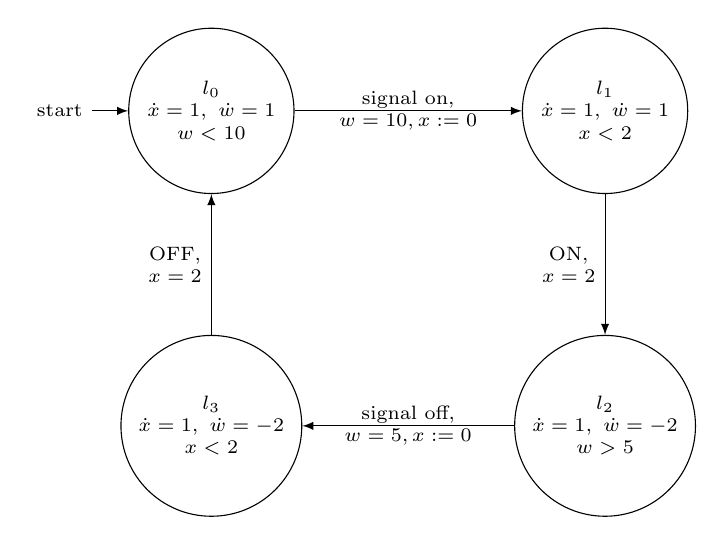
\begin{tikzpicture}[node distance=5cm]
            \node[state,initial] (s0) {$l_{0}$ \\ $\dot{x}=1,\ \dot{w}=1$ \\ $w<10$};
            \node[state] (s1) [right of = s0] {$l_{1}$ \\ $\dot{x}=1,\ \dot{w}=1$ \\ $x<2$};
            \node[state] (s2) [below of = s1,node distance=4cm] {$l_{2}$ \\ $\dot{x}=1,\ \dot{w}=-2$ \\ $w>5$};
            \node[state] (s3) [below of = s0,node distance=4cm] {$l_{3}$ \\ $\dot{x}=1,\ \dot{w}=-2$ \\ $x<2$};
            \path[->] (s0) edge node {signal on, \\ $w=10,x:=0$} (s1)
                (s1) edge node [left] {ON, \\ $x=2$} (s2)
                (s2) edge node {signal off, \\ $w=5,x:=0$} (s3)
                (s3) edge node [left] {OFF, \\ $x=2$} (s0);
        \end{tikzpicture}
        \caption{Linear Hybrid Automaton of a water-level monitor.}
        \label{fig:exwaterlevel}
    \end{center}
\end{figure}
\end{ex}
Another way of looking at linear hybrid automata is as this type being a special case of rectangular automata.

\begin{defi}[Linear Hybrid Automaton \cite{Alur2000}]
A \emph{linear hybrid automaton} is a rectangular automaton where
\begin{itemize}
    \item{for each $\ell\in L$, $Init(\ell)$ is a singleton or empty, $R^{\ell}=f(\ell)(x)$ is a singleton set, $\forall x\in V$,}
    \item{for each edge $e\in E$ the guard set $g(e)$ and the reset map $r(e)$ are singleton sets.}
\end{itemize}
\end{defi}

\subsection{Timed Automata}
Timed automata were originally introduced as timed B\"{u}chi Automata \cite{Alur1990,Alur1994}, and can be seen as a special case of linear hybrid automata.

\begin{defi}[Timed Automaton \cite{Lygeros2004}]
A \emph{timed automaton} is a linear hybrid automaton where the flow condition in all modes is of the form $\dot{x}=1$, $\forall x\in V$.
\end{defi}

\begin{ex}[Timed Automaton Example \cite{Alur2000}]
The automaton in Figure~\ref{fig:extime} is a generic example of a timed automaton. The automaton is similar to the example of a rectangular automaton in Figure~\ref{fig:exrect}. Noticeable are the differential equations which in the timed automaton ate all of the form $\dot{x}=1$.

\begin{figure}[H]
    \begin{center}
        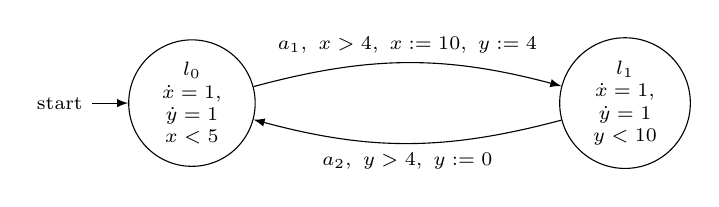
\begin{tikzpicture}[node distance=5.5cm]
            \node [state,initial] (s0) {$l_{0}$ \\ $\dot{x}=1,$\\$\dot{y}=1$ \\ $x<5$};
            \node [state] (s1) [right of = s0] {$l_{1}$ \\ $\dot{x}=1,$\\$\dot{y}=1$ \\ $y<10$};
            \path[->] (s0) edge [bend left=15] node [above] {$a_{1},\ x>4,\ x:=10,\ y:=4$} (s1)
                (s1) edge [bend left=15] node [below] {$a_{2},\ y>4,\ y:=0$} (s0);
        \end{tikzpicture}
        \caption{Example of a timed automaton.}
        \label{fig:extime}
    \end{center}
\end{figure}
\end{ex}


%%%%%%%%%%%%%%%%%%%%%%%%%%%%%%%%%%%%%%%%%%%%%%%%%%%%%%%%%%%%%%%%%%%%%%%%%%%%%%%%%%%%%%%%%%%%%%%%%%%
%%%%%%%%%%%%%%%%%%%%%%%%%%%%%%%%%%%%%%%%%%%%%%%%%%%%%%%%%%%%%%%%%%%%%%%%%%%%%%%%%%%%%%%%%%%%%%%%%%%
%%% STOCHASTIC HA
%%%%%%%%%%%%%%%%%%%%%%%%%%%%%%%%%%%%%%%%%%%%%%%%%%%%%%%%%%%%%%%%%%%%%%%%%%%%%%%%%%%%%%%%%%%%%%%%%%%
%%%%%%%%%%%%%%%%%%%%%%%%%%%%%%%%%%%%%%%%%%%%%%%%%%%%%%%%%%%%%%%%%%%%%%%%%%%%%%%%%%%%%%%%%%%%%%%%%%%
\subsection{Stochastic Hybrid Automata}

One type of stochastic hybrid automata is governed by stochastic behaviour of the continuous variables in each mode, rather than deterministic behaviour. So the flow of the continuous variables in the modes evolves through stochastic differential equations
\[
\dot{x} = f(\ell)(x) + dB_{t},
\]
where $B_{t}$ can be seen as the standard Brownian motion in $\mathbb{R}$ \cite{Hu2000}, or as a $\mathbb{R}^{n}$ valued Wiener process \cite{Koutsoukos2006}.

Further, the transitions between the modes will be probabilistic.

\begin{defi}[Stochastic Hybrid Automaton \cite{Hu2000}]
A \emph{stochastic hybrid automaton} is a hybrid automaton $\mathcal{A}=(V,L,A,Init,Inv,E,f)$ where
\begin{itemize}
    \item{for each edge $e\in E$ the guard $g(e)$ is a measurable subset of $\delta Inv$, or empty,}
    \item{the reset map $r$ is changed to be $r : E \rightarrow \mathcal{P}(val(V))$, such that is assigns each edge $(\ell,a,\ell')\in E$ a reset probability kernel on $val(V)$ concentrated on $Inv(\ell')$. Further, for any measurable set $M\subset Inv(\ell')$, $r(e)(M)$ is a measurable function.}
\end{itemize}
\end{defi}

\begin{ex}[Car Chase \cite{Hu2000}]
Imagine two cars $x_{1}$ and $x_{2}$ on a straight road. Both cars drive in the same direction, where the task for $x_{1}$ is to catch up with $x_{2}$ (which is driving at a constant speed) up to given distance, keep following, if $x_{1}$ gets too close, $x_{1}$ breaks and falls back. The motion of both cars is stochastic, due to many unknown factors such as the road condition or the environment. We can abstract the stochastic behaviour away from the motion of $x_{2}$ as we are modeling the behaviour of $x_{1}$. The distance between the two cars is $\Delta x$. There are multiple distance thresholds we consider $d_{0}>d_{1}>d_{2}>d_{3}>0$ which are in order, post breaking distance, chasing distance, keeping distance and being too close. Figure~\ref{fig:excar} shows the three modes of the scenario, chasing, keeping up and breaking. We denote the probability of $x_{1}$ falling behind $x_{2}$ further than the the keeping up distance by $p$, so the probability of being too close to $x_{2}$ is $1-p$.
\begin{figure}[H]
    \begin{center}
        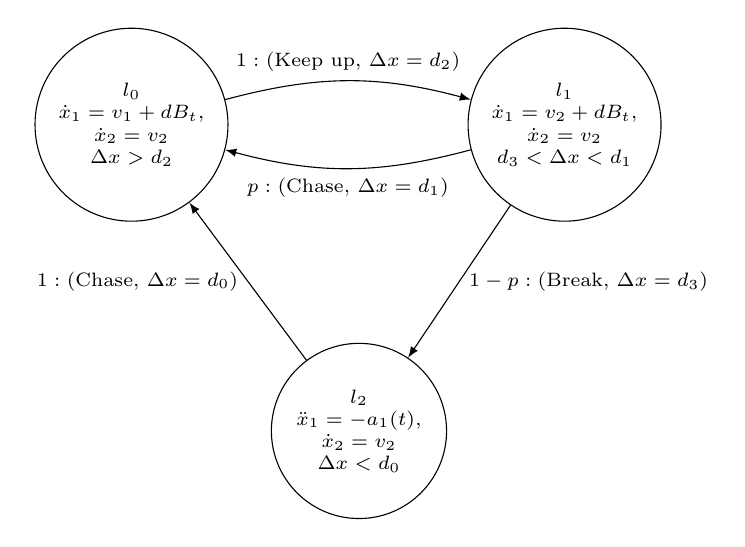
\begin{tikzpicture}[node distance=5.5cm]
            \node [state] (s0) {$l_{0}$\\ $\dot{x}_{1}=v_{1}+dB_{t},$\\$\dot{x}_{2}=v_{2}$\\ $\Delta x>d_{2}$};
            \node [state] (s1) [right of = s0] {$l_{1}$\\ $\dot{x}_{1}=v_{2}+dB_{t},$\\$\dot{x}_{2}=v_{2}$\\ $d_{3}<\Delta x<d_{1}$};
            \node [state] (s2) [below right of = s0,xshift=-1cm] {$l_{2}$\\ $\ddot{x}_{1}=-a_{1}(t),$\\$\dot{x}_{2}=v_{2}$\\ $\Delta x<d_{0}$};
            \path[->] (s0) edge [bend left=15] node [above] {$1:($Keep up, $\Delta x=d_{2})$} (s1)
                (s1) edge [bend left=15] node [below] {$p:($Chase, $\Delta x=d_{1})$} (s0)
                    edge node [right] {$1-p:($Break, $\Delta x=d_{3})$} (s2)
                (s2) edge node [left] {$1:($Chase, $\Delta x=d_{0})$} (s0);
        \end{tikzpicture}
        \caption{Example of a simplistic car chase as a stochastic hybrid automaton.}
        \label{fig:excar}
    \end{center}
\end{figure}
\end{ex}

Another type of stochastic hybrid systems have just probabilistic discrete transitions between the modes, while the behaviour of the continuous variables inside the modes can be deterministic. This type of hybrid automaton is called probabilistic.

\begin{defi}[Probabilistic Hybrid Automaton \cite{Hahn2011}]
A hybrid automaton $\mathcal{A}=(V,L,A,Init,Inv,E,f)$ is \emph{probabilistic} if we define a \emph{transition function} on the edges between the modes $t : L\times A \rightarrow \mathcal{P}(L)$, where $\mathcal{P}(L)$ is a distribution over $L$, and the guard and reset maps, $g(\ell,a,\ell'),\ r(\ell,a,\ell')$  are defined over the set of edges $E \subseteq L \times A \times L$ if $t(\ell,a)=\mathcal{P}(\ell')\neq 0$.
\end{defi}


%%%%%%%%%%%%%%%%%%%%%%%%%%%%%%%%%%%%%%%%%%%%%%%%%%%%%%%%%%%%%%%%%%%%%%%%%%%%%%%%%%%%%%%%%%%%%%%%%%%
%%%%%%%%%%%%%%%%%%%%%%%%%%%%%%%%%%%%%%%%%%%%%%%%%%%%%%%%%%%%%%%%%%%%%%%%%%%%%%%%%%%%%%%%%%%%%%%%%%%
%%% O MIN HA
%%%%%%%%%%%%%%%%%%%%%%%%%%%%%%%%%%%%%%%%%%%%%%%%%%%%%%%%%%%%%%%%%%%%%%%%%%%%%%%%%%%%%%%%%%%%%%%%%%%
%%%%%%%%%%%%%%%%%%%%%%%%%%%%%%%%%%%%%%%%%%%%%%%%%%%%%%%%%%%%%%%%%%%%%%%%%%%%%%%%%%%%%%%%%%%%%%%%%%%
\subsection{Order-Minimal Hybrid Automata}
The idea behind order-minimal hybrid automata is to limit the discrete transitions, rather than the continuous flow. With this restriction it can be easier to abstract the hybrid system.

%To introduce the notion of order-minimality, first we need to consider a few definitions from formal language theory.

%\begin{defi}[Theory]

%\end{defi}

\begin{defi}[Order-Minimal Theory \cite{Lafferriere1999}]
The theory over the reals $Th(\mathbb{R})$ is \emph{o-minimal} (order-minimal) if every definable subset of $\mathbb{R}$ is a finite union of points and intervals (possibly unbounded).
\end{defi}

\begin{defi}[Order-Minimal Hybrid Automaton \cite{G.Lafferiere2000}]
A hybrid system $\mathcal{A}=(V,L,A,Init,Inv,E,f)$ is called \emph{o-minimal} if
\begin{itemize}
    \item{for each $\ell\in L$, the flow $f(\ell)$ is a complete differential function (defined for all time);}
    \item{for each $e\in E$, the reset map $r(e)$ is a piecewise constant but set valued map, with a finite number of pieces;}
    \item{for each $\ell\in L$ and all $e\in E$, $Inv(\ell),\ Init(\ell),\ , g(e),\ f(\ell)$ are definable over the same o-minimal theory over $\mathbb{R}$.}
\end{itemize}
\end{defi}

\begin{ex}[Timed Digital Code \cite{Brihaye2005}]
In this example we model a door which is locked and alarmed. To unlock it safely the user has to swipe a card $c$ and then enter the correct passcode $w$. The passcode is $ABC$ and the user has one time unit $t$ for each letter. Should they enter a wrong letter or not within the given time, the alarm will go off. This example can be modelled as a o-minimal hybrid automaton as in Figure~\ref{fig:expass}.

\begin{figure}[H]
    \begin{center}
        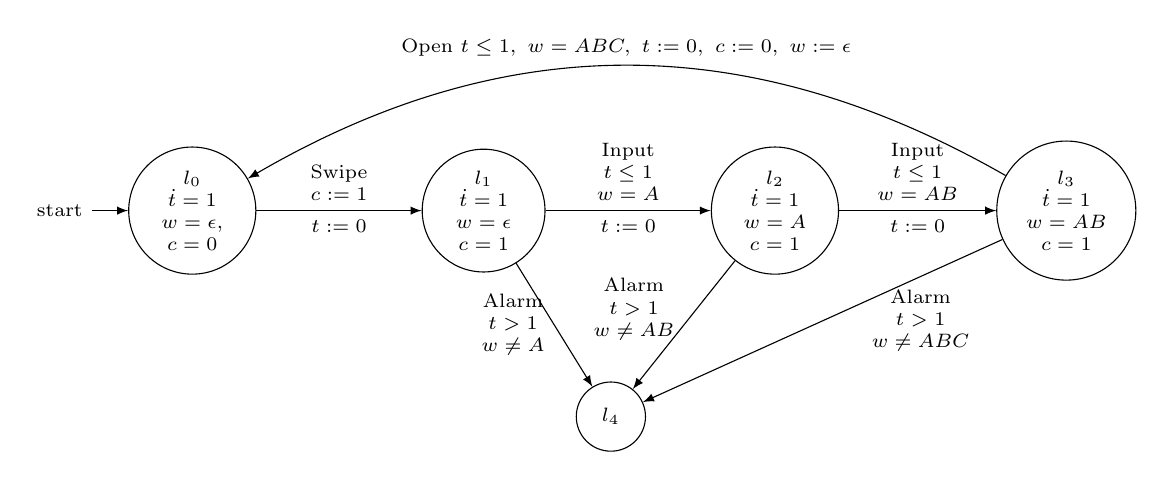
\begin{tikzpicture}[node distance=3.7cm]
            \node [state,initial] (s0) {$l_{0}$\\$\dot{t}=1$\\$w=\epsilon,$\\$c=0$};
            \node [state] (s1) [right of = s0] {$l_{1}$\\$\dot{t}=1$\\$w=\epsilon$\\$c=1$};
            \node [state] (s2) [right of = s1] {$l_{2}$\\$\dot{t}=1$\\$w=A$\\$c=1$};
            \node [state] (s3) [right of = s2] {$l_{3}$\\$\dot{t}=1$\\$w=AB$\\$c=1$};
            \node [state] (s4) [below right of = s1,xshift=-1cm] {$l_{4}$};

            \path[->] (s0) edge node [above] {Swipe\\$c:=1$} node [below] {$t:=0$} (s1)
                (s1) edge node [above] {Input\\$t\leq1$\\$w=A$} node [below] {$t:=0$} (s2)
                    edge node [left] {Alarm\\$t>1$\\$w\neq A$} (s4)
                (s2) edge node [above] {Input\\$t\leq1$\\$w=AB$} node [below] {$t:=0$} (s3)
                    edge node [left,yshift=2mm] {Alarm\\$t>1$\\$w\neq AB$} (s4)
                (s3) edge [bend right] node [above] {Open $t\leq1,\ w=ABC,\ t:=0,\ c:=0,\ w:=\epsilon$} (s0)
                    edge node [right,xshift=5mm] {Alarm\\$t>1$\\$w\neq ABC$} (s4);

        \end{tikzpicture}
        \caption{Example of a secured door, with timed passcode entry.}
        \label{fig:expass}
    \end{center}
\end{figure}
\end{ex}

Rectangular Set: conjunction of $x\sim c$, where $x\in \val(C)$, $c\in\mathbb{Q}$, and $\sim\in\{<,\leq,=,\geq,>\}$; $B=B_{1}\times\cdots\times B_{n}\subseteq \mathbb{R}^{n}$.

Linear Term: $k_{0}x_{0}+\cdots+k_{n}x_{n}$, where $k_{0},\ldots,k_{n}\in \mathbb{Z}$, $x_{0},\ldots,x_{n}\in V$, $\val(V)\in\mathbb{R}^{n}$.
Linear Expression: $\tau_{1}\sim\tau_{2}$, where $\sim\in\{<,\leq,=,\geq,>\}$ and $\tau_{1},\tau_{2}$ are linear terms.



\begin{table}
\begin{center}
\begin{tabular}{|l|l|l|l|l|}\hline
Type & $Init$, $Inv$ & $g$ & $r$ & $f$ \\ \hline
Rectangular & Rectangular & Rectangular & Rectangular & $f(\ell)(x) = B^{\ell}$ \\ \hline
Linear & Linear & Linear  & Linear  & $f(\ell)(x)=k$ \\ \hline
Timed & Linear & Linear & Linear & $f(\ell)(x)=1, \forall x$ \\ \hline
Stochastic &  &  &  & \\ \hline
O-Minimal &  &  &  & \\ \hline
\end{tabular}
\label{tab:hasummary}
\caption{Summary of the presented types of hybrid systems.}
\end{center}
\end{table}
%\cite{Alur1995a,Amin2006,Alur1993,Alur2011a,Henzinger2000,Maler2014a,Nicollin1993,Platzer2011a,Raskin2005,Tabuada,Fehnker2004,Tomlin2003,Alur1997,Asarin1997}

%\cite{Alur2011a} mentions some abstractions  (flowpipe, simulation, phase portrait)

%\cite{Henzinger2000} covers some abstraction techniques with refs (discrete, bisimulation, $\mu$)

%\cite{Maler2014a} contains some refs to different types of abstr.

%\cite{Asarin1997} timed aut abstraction using numberical decision diagram

%\subsection{Applications}
%\cite{Chaimowicz2003} in robotic cooperation

%\cite{Dennis2013a} more robotic applications and some refs to abstractions.

%\cite{Fehnker2004} contains benchmarks and uses both d/dt anf charon.

%\cite{Tomlin2003} with tools


\section{Abstractions}
\label{sec:abs}
There are different types of abstraction techniques that can be applied to hybrid automata, we will discuss these in the sections below. What these techniques have in common is that they construct a discrete \emph{transition system} and they show that the abstraction preserves the properties of the original system. Some of the techniques use the properties to build partitions of the hybrid system, which then are abstracted.

\begin{defi}[Transition System \cite{Alur2000}]
A \emph{transition system} $\mathcal{T}=(Q,Q_{0},\Pi,t,\models)$ consists of
\begin{description}
    \item[$Q$]{the finite set of states;}
    \item[$Q_{0}\subseteq Q$]{the set of initial states;}
    \item[$\Pi$]{the set of propositions;}
    \item[$t \subseteq Q\times Q$]{a transition function;}
    \item[$\models\subseteq Q\times\Pi$]{a satisfaction function.}
\end{description}
\end{defi}

The \emph{properties} of a system are desired specifications, such as avoiding an unsafe set of states, that the system satisfies. Properties are used to formally verify the system and are described using logical formulae built from atomic propositions.

We denote by $\llbracket \pi \rrbracket = \{ q\in Q : q\models \pi\}$ the set of states satisfying the property $\pi$.

\begin{defi}[Linear Temporal Logic]
The formulae of \emph{linear temporal logic} (LTL) are defined recursively
\begin{description}
    \item[Propositions]{Every atomic proposition $\pi$ is a formula.}
    \item[Formulas]{If $\phi_{1}$ and $\phi_{2}$ are formulae then so are the following;
        \[
        \phi_{1} \lor \phi_{2},\ \ \phi_{1} \land \phi_{2}, \ \ \lnot \phi_{1}, \ \
        \phi_{1} \Rightarrow \phi_{2},\ \ \phi_{1} \Leftrightarrow \phi_{2}, \ \ \bigcirc \phi_{1}, \ \ \phi_{1} \until \phi_{2}, \ \ \lozenge \phi_{1}, \ \ \square \phi_{1}.
        \]}
\end{description}
\end{defi}
Where the formulae are interpreted over infinite words of propositions. Let $w=\Pi_{0}\Pi_{1}\ldots$ be a word with $\Pi_{i}$ being a set of propositions, then the satisfaction of a proposition $\pi$ at position $i\in \mathbb{N}$ of $w$ is denoted by $(w,i)\models_{L} \pi$ and holds if and only if $\pi \in \Pi_{i}$. Note that $\models_{L}$ is not the satisfaction relation $\models$ of a transition system.

\begin{defi}[Semantics of LTL]
Let $\phi_{1},\phi_{2}$ be LTL formulae, $w$ a word of propositions, and $i\in\mathbb{N}$. The semantics of any LTL formula is defined recursively as
\begin{itemize}
    \item{$(w,i)\models_{L}\phi_{1}\lor\phi_{2}$ if either $(w,i)\models_{L}\phi_{1}$ or $(w,i)\models_{L}\phi_{2}$;}
    \item{$(w,i)\models_{L}\phi_{1}\land\phi_{2}$ if both $(w,i)\models_{L}\phi_{1}$ and $(w,i)\models_{L}\phi_{2}$;}
    \item{$(w,i)\models_{L}\lnot\phi_{1}$ if $(w,i)\not\models_{L}\phi_{1}$;}
    \item{$(w,i)\models_{L}\phi_{1}\Rightarrow\phi_{2}$ if $(w,i)\models_{L}\lnot\phi_{1} \land \phi_{2}$;}
    \item{$(w,i)\models_{L}\phi_{1}\Leftrightarrow\phi_{2}$ if $(w,i)\models_{L}(\phi_{1}\Rightarrow\phi_{2})\land(\phi_{2}\Rightarrow\phi_{1})$;}
    \item{$(w,i)\models_{L}\bigcirc\phi_{1}$ if $(w,i+1)\models_{L}\phi_{1}$;}
    \item{$(w,i)\models_{L}\phi_{1}\until\phi_{2}$ if there is $j\geq i$ such that $(w,j)\models_{L}\phi_{2}$ and for all $i\leq k < j$ $(w,k)\models_{L}\phi_{1}$;}
    \item{$(w,i)\models_{L}\lozenge\phi_{1}$ if $(w,i)\models_{L}true\until\phi_{1}$;}
    \item{$(w,i)\models_{L}\square\phi_{1}$ if $(w,i)\models_{L}\lnot\lozenge\lnot\phi_{1}$.}
\end{itemize}
\end{defi}

The \emph{next} operator $\bigcirc\phi$ holds for a word $\Pi_{0}\Pi_{1}\Pi_{2}\ldots$ if and only if $\phi$ holds for $\Pi_{1}\Pi_{2}\ldots$. The \emph{until} operator $\phi_{1}\until\phi_{2}$ describes that $\phi_{1}$ is true until $\phi_{2}$ becomes true. The \emph{eventually} operator $\lozenge\phi$ indicates that $\phi$ will be true at some point in $w$. The \emph{always} operator $\square\phi$ describes that $\phi$ must always be true in a word.

We can extend LTL to include existential quantifiers. These types of quantifiers are used in property formulations of transition systems and the satisfaction relation of correlates to the satisfaction relation of this extended logic.

\begin{defi}[Computational Tree Logic]
    The formulae of \emph{Computational temporal logic} (CTL) are defined recursively
\begin{description}
    \item[Propositions]{Every atomic proposition $\pi$ is a formula.}
    \item[Formulas]{If $\phi_{1}$ and $\phi_{2}$ are formulae then so are the following;
        \[
        \phi_{1} \lor \phi_{2},\ \ \phi_{1} \land \phi_{2}, \ \ \lnot \phi_{1}, \ \
        \phi_{1} \Rightarrow \phi_{2},\ \ \phi_{1} \Leftrightarrow \phi_{2}, \ \
        \exists\bigcirc \phi_{1}, \ \ \phi_{1} \exists\until \phi_{2}, \ \
        \exists\lozenge \phi_{1}, \ \ \exists\square \phi_{1}, \ \ \forall\bigcirc \phi_{1}, \ \
        \forall\lozenge \phi_{1}, \ \ \forall\square \phi_{1}.
        \]}
\end{description}
\end{defi}

The difference between LTL and CTL semantics is that LTL is interpreted over words, whereas CTL is interpreted over trees generated by trajectories from a given state of a transition system. So a transition system $\mathcal{T}$ satisfies a proposition $\pi$ if there is a state $q_{0}\in Q$ in $\mathcal{T}$ such that $q_{0}\models \pi$.
\begin{defi}[Semantics of CTL]
Let $q_{0}\in Q$ be a state of a transition system $\mathcal{T}$, and $\phi_{1},\phi_{2}$ CTL formulae, then the semantics of CTL is defined as
\begin{itemize}
    \item{$q_{0}\models\phi_{1}\lor\phi_{2}$ if either $q_{0}\models\phi_{1}$ or $q_{0}\models\phi_{2}$;}
    \item{$q_{0}\models\phi_{1}\land\phi_{2}$ if both $q_{0}\models\phi_{1}$ and $q_{0}\models\phi_{2}$;}
    \item{$q_{0}\models\lnot\phi_{1}$ if $q_{0}\not\models\phi_{1}$;}
    \item{$q_{0}\models\phi_{1}\Rightarrow\phi_{2}$ if $q_{0}\models\lnot\phi_{1} \land \phi_{2}$;}
    \item{$q_{0}\models\phi_{1}\Leftrightarrow\phi_{2}$ if $q_{0}\models(\phi_{1}\Rightarrow\phi_{2})\land(\phi_{2}\Rightarrow\phi_{1})$;}
    \item{$q_{0}\models\exists\bigcirc\phi_{1}$ if $\exists q_{1}\in Q$ such that
    $t(q_{0})=q_{1}$ and $q_{1}\models \phi_{1}$;}
    \item{$q_{0}\models\phi_{1}\exists\until\phi_{2}$ if $\exists q_{0}q_{1}q_{2}\ldots$ a trajectory generated from $q_{0}$ such that $q_{i}\models \phi_{2}$ for some $i\geq 0$ and for all $0\leq j < i$, $q_{j}\models \phi_{1}$;}
    \item{$q_{0}\models\exists\lozenge\phi_{1}$ if $q_{0}\models true\ \exists\until \phi_{1}$;}
    \item{$q_{0}\models\exists\square\phi_{1}$ if $\exists q_{0}q_{1}q_{2}\ldots$ generated from $q_{0}$ such that $\forall i\geq 0$ $q_{i}\models\phi_{1}$;}

    \item{$q_{0}\models\forall\bigcirc\phi_{1}$ if $q_{0}\models\lnot\exists\bigcirc\lnot\phi_{1}$;}
    \item{$q_{0}\models\forall\lozenge\phi_{1}$ if $q_{0}\models\lnot\exists\square\lnot\phi_{1}$;}
    \item{$q_{0}\models\forall\square\phi_{1}$ if $q_{0}\models\lnot\exists\lozenge\lnot\phi_{1}$.}
\end{itemize}
\end{defi}

The temporal operators $\exists\bigcirc, \exists\until, \exists\lozenge$ and $\exists\square$ are called \emph{possibly next}, \emph{possibly always}, \emph{possibly until}, and \emph{possibly eventually} respectively and they refer to the existence of a trajectory starting at a given state. On the other hand, the operators $\forall\bigcirc$ (inevitably next), $\forall\lozenge$ (inevitably eventually) and $\forall\square$ (inevitably always) refer to all trajectories from a given state.

In general we can say that a transition system $\mathcal{T}$ \emph{satisfies} a CTL formula $\phi$ if some initial state of $\mathcal{T}$ satisfies $\phi$.

\subsection{General Verification Problems}
There are general questions that we can ask of a system which we are looking to be verified for example, we reach all possible states of the system.

\begin{prob}[Reachability Problem \cite{Henzinger2000}]
\label{prob:reach}
Given a hybrid automaton $\mathcal{A}$ and a proposition $\phi$. Is there a trajectory in the hybrid automaton that starts in an initial state and reaches a state $(l_{i},v)\in L\times\val(V)$ such that $(l_{i},v)\models\phi$?
\end{prob}

\begin{prob}[Emptiness Problem \cite{Henzinger2000}]
\label{prob:empty}
Given a hybrid automaton $\mathcal{A}$, is there a divergent trajectory starting in an initial state?
\end{prob}

%A \emph{timed trace} in a hybrid automaton is
%\begin{prob}[Timed Trace Inclusion Problem \cite{Henzinger2000}]
%\label{prob:time}
%Given two hybrid automata $\mathcal{A}_{1}$ and $\mathcal{A}_{2}$, is every timed trace in $\mathcal{A}_{1}$ also a timed trace in $\mathcal{A}_{2}$
%\end{prob}

\begin{prob}[LTL Model Checking Problem \cite{Alur2000}]
\label{prob:ltl}
Given a hybrid automaton $\mathcal{A}$ and a LTL formula $\phi$ , determine if $\mathcal{A}$ satisfies $\phi$.
\end{prob}

\begin{prob}[CTL Model Checking Problem \cite{Alur2000}]
\label{prob:ctl}
Given a hybrid automaton $\mathcal{A}$ and a CTL formula $\phi$ , determine if $\mathcal{A}$ satisfies $\phi$.
\end{prob}



\subsection{Running Example}
Figure~\ref{fig:UAV} is the hybrid automaton which will be abstracted in with each technique. Some abstractions call for a specific type of hybrid automaton, we will adjust the components accordingly and draw the new automaton.

The example hybrid system that we use is a simplified scenario of an unmanned aerial vehicle (UAV) taking off to height $H_{1}$, move forward over a distance of $M$ or ascend higher to height $H_{2}$. The UAV will not start landing until it has reached the distance $M$.
There are many different properties we can investigate in this hybrid system, we will consider the following three questions:
\begin{itemize}
    \item{Will the UAV take off, fly at height $H_{1}$ before landing?}
    \item{Will the UAV ever reach height $H_{2}$?}
    \item{Will the UAV fly forward, then go higher and then fly on?}
\end{itemize}
\begin{figure}[H]
    \begin{center}
        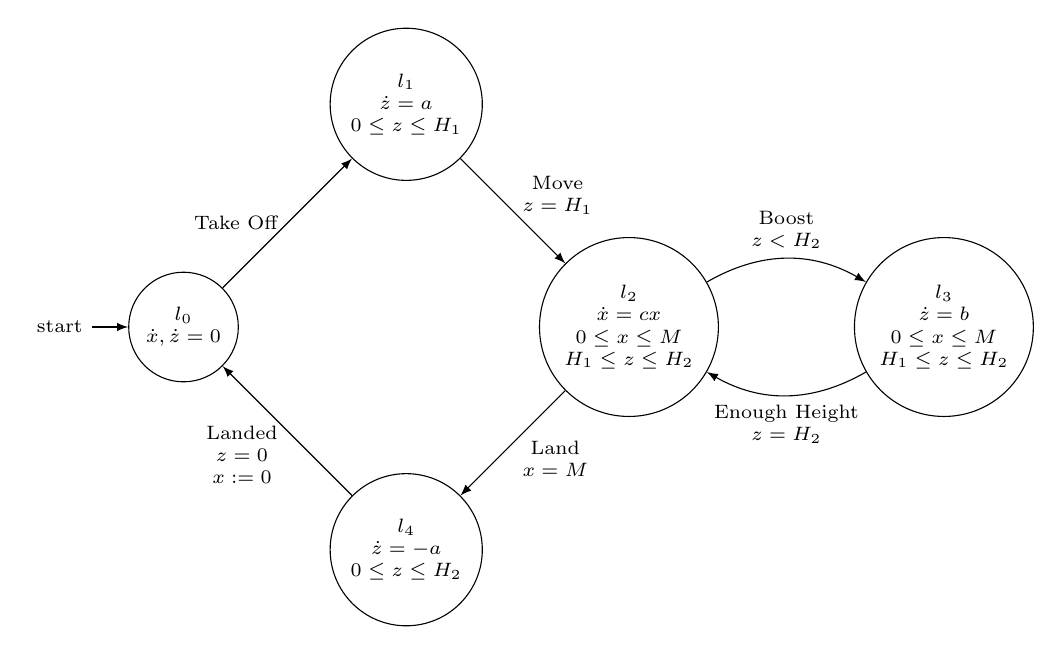
\begin{tikzpicture}[node distance=4cm]
            \node [state,initial] (s0) {$l_{0}$\\$\dot{x},\dot{z}=0$};
            \node [state] (s1) [above right of = s0] {$l_{1}$\\$\dot{z}=a$\\$0\leq z\leq H_{1}$};
            \node [state] (s2) [below right of = s1] {$l_{2}$\\$\dot{x}=cx$\\$0\leq x\leq M$\\$H_{1}\leq z\leq H_{2}$};
            \node [state] (s3) [below right of = s0] {$l_{4}$\\$\dot{z}=-a$\\$0\leq z\leq H_{2}$};
            \node [state] (s4) [right of = s2] {$l_{3}$\\$\dot{z}=b$\\$0\leq x \leq M$\\$H_{1}\leq z\leq H_{2}$};

            \path[->] (s0) edge node [left] {Take Off} (s1)
                (s1) edge node [right,yshift=2mm] {Move \\ $z=H_{1}$} (s2)
                (s2) edge node [right,yshift=-2mm] {Land \\ $x=M$} (s3)
                    edge [bend left] node [above] {Boost \\ $z < H_{2}$} (s4)
                (s3) edge node [left,yshift=-3mm] {Landed \\ $z=0$ \\ $x:=0$} (s0)
                (s4) edge [bend left] node [below] {Enough Height \\ $z=H_{2}$} (s2);
        \end{tikzpicture}
        \caption{Hybrid Automaton of a UAV.}
        \label{fig:UAV}
    \end{center}
\end{figure}

Formally, the hybrid automaton in Figure~\ref{fig:UAV} consists of the following:
\begin{align*}
V & = \{x,z\} \text{ with } \val(V)\subseteq\mathbb{R}^{2} \\
L & = \{l_{0},l_{1}, l_{2}, l_{3}, l_{4}\} \\
A & = \{ \text{Take Off, Move, Boost, Enough Height, Land, Landed} \} \\
Init & = \{(l_{0},(0,0))\} \\
Inv(l_{0}) & = (0,0),\ \ Inv(l_{1}) = (0,[0,H_{1}]),\ \ Inv(l_{2}) = ([0,M],[H_{1},H_{2}]),\\
Inv(l_{3}) & = ([0,M],[H_{1},H_{2}]), \ \ Inv(l_{4})=([0,M],[0,H_{2}]) \\
f(l_{0}) &=(\dot{x}=0,\dot{z}=0),\ \ f(l_{1})=(\dot{x}=0,\dot{z}=a),\ \ f(l_{2})=(\dot{x}=cx,\dot{z}=0),\\
f(l_{3}) &=(\dot{x}=0,\dot{z}=b), \ \ f(l_{4}) = (\dot{x}=0,\dot{z}=-a) \\
E & = \{e_{1}=(l_{0},\text{Take Off},l_{1}),\ e_{2}=(l_{1},\text{Move},l_{2}),\  e_{3}=(l_{2},\text{Boost},l_{3}),\\
& e_{4}=(l_{3},\text{Enough Height},l_{2}),\  e_{5}=(l_{2},\text{Land},l_{4}),\ e_{6}=(l_{4},\text{Landed},l_{0})\} \\
g(e_{1}) & =\emptyset,\ \ g(e_{2})=(\emptyset,H_{1}),\ \ g(e_{3})=\emptyset, \ \ g(e_{4})=(\emptyset,H_{2}),\ \ g(e_{5})=(M, \emptyset),\ \ g(e_{6})=(\emptyset,0) \\
r(e_{1}) & =(x,z),\ \ r(e_{2})=(x,z),\ \ r(e_{3})=(x,z),\ \ r(e_{4})=(x,z),\ \ r(e_{5}) = (x,z),\ \ r(e_{6})=(0,z) \\
\end{align*}

The three properties can be written in CTL as
\[
(x=0 \land z=0) \until (x=0 \land z>0) \until (z=H_{1}) \until (z<H_{1})
\]
\[
\exists\lozenge (z=H_{2})
\]
\[
\forall \lozenge (z>0 \until \bigcirc z=0)
\]

\subsection{Discrete Abstraction}
\label{sec:disc}
The discrete abstraction of a hybrid automaton consists of finding a suitable transition system. The checking of whether the defined transition system is equivalent to the hybrid automaton is done through algorithmic evaluation of the behaviour of the continuous flows, as the discrete jumps of the hybrid automaton are preserved.

A hybrid system $\mathcal{A}=(V,L,A,Init,Inv,E,f)$ generates a transition system $\mathcal{T}_{\Sigma,\mathcal{A}}=(Q,Q_{0},\Pi,t,\models)$ according to a finite set of subsets of $\mathbb{R}^{n}$, denoted $\Sigma$, where $n$ is the number of continuous variables \cite{Alur2000}. Then
\begin{itemize}
\item{$Q=L\times \val(V)$ is the set of states;}
\item{$Q_{0}=Init$ is the set of initial states;}
\item{$\Pi=L\cup\Sigma$ is the set of propositions;}
\item{$(\ell,x)\models\pi$ is the satisfaction relation where $\ell\in L$ and then $\pi\in L$ if and only if $\ell = \pi$, or $\pi\in\Sigma$ if and only if $x\in\pi$;}
\item{$t=(\bigcup_{e\in E}\overset{e}{\rightarrow})\cup \overset{\tau}{\rightarrow}$ is the
transition function, with $\overset{e}{\rightarrow}$ being the discrete transitions, which are
defined as $(\ell,x)\overset{e}{\rightarrow}(\ell',x')$ for $e=(\ell,a,\ell')\in E$ for any
$a\in A$ if and only if $x\in g(e)$ and $x' \in r(e)$ and $\overset{\tau}{\rightarrow}$ are
continuous transitions, which are defined as
$(\ell_{1},x_{1})\overset{\tau}{\rightarrow}(\ell_{2},x_{2})$ if and only if $\ell_{1}=\ell_{2}$,
and $\exists \delta \in \mathbb{R}^{+}\setminus\{ 0\}$ and there is a differentiable curve
$x:[0,\delta]\rightarrow \mathbb{R}^{n}$ with $x(0)=x_{1}$, $x(\delta)=x_{2}$ and
$\forall t\in[0,\delta]$ $x(t)\in Inv(\ell_{1})$, $\forall t\in (0,\delta)$
$\dot{x}(t)\in f(\ell_{1})$ .}
\end{itemize}


We need to show that the constructed transition system, is still preserving the properties accordingly. For that we are looking at bisimulations to show that in fact we can still check CTL or LTL properties, through partitioning the state space.

\begin{defi}[Equivalence Relation on States]
An \emph{equivalence relation} $\sim\subseteq Q\times Q$ on the state space of a transition system $\mathcal{T}$ is proposition preserving if for all state $p,q\in Q$ and all propositions $\pi\in\Pi$, if $p\sim q$ and $p\models\pi$, then $q\models\pi$.
\end{defi}

So $\llbracket \pi\rrbracket$ the set of states satisfying the property $\pi$ can be seen as the union of equivalence classes.

\begin{defi}[Quotient Transition System]
Given a proposition preserving equivalence relation $\sim$, a \emph{quotient transition system} $\mathcal{T}/_{\sim}=(Q/_{\sim},Q_{0}/_{\sim},\Pi,t_{\sim},\models_{\sim})$ consists of
\begin{itemize}
\item{$Q/_{\sim}$ the quotient space, the set of equivalence classes;}
\item{$t_{\sim}$ is the transition relation, for $P_{1},P_{2}\in Q/_{\sim}$ we have $t_{\sim}(P_{1})=P_{2}$ if and only if there exists two states $q_{1}\in P_{1}$ and $q_{2}\in P_{2}$ such that $t(q_{1})=q_{2}$.}
\item{$\models_{\sim}$ is the satisfaction relation, where for $P\in Q/_{\sim}$ $P\models_{\sim}\pi$ if and only if $\exists p\in P$ such that $p\models \pi$.}
\end{itemize}
\end{defi}

For any set of states $P$ let $P/_{\sim}$ denote the collection of all equivalence classes that intersect $P$.

\begin{defi}[Bisimulation \cite{Roggenbach2000}]
Let $\mathcal{T}=(Q,Q_{0},\Pi,t,\models)$ be a transition system. A proposition preserving equivalence relation $\sim_{B}$ on $Q$ is a \emph{bisimulation} of $\mathcal{T}$ if for all states $p,q\in Q$ if $p \sim_{B} q$, then for all states $p'\in Q$ if $t(p)=p'$, $\exists q'\in Q$ such that $t(q)=q'$ and $p'\sim_{B} q'$.
\end{defi}

If $\sim_{B}$ is a bisimulation, then the quotient transition system $\mathcal{T}/_{\sim_{B}}$is called a \emph{bisimulation quotient} of $\mathcal{T}$.

\begin{thm}[\cite{Browne1988}]
Let $\mathcal{T}$ be a transition system and let $\sim_{B}$ be a bisimulation of $\mathcal{T}$. Then $\mathcal{T}$ satisfies the CTL formula $\phi$ if and only if the bisimulation quotient $\mathcal{T}/_{\sim_{B}}$ satisfies $\phi$.
\end{thm}

We can construct the bisimulation quotient algorithmically.

\begin{algorithm}[H]
$Q/_{\sim_{B}} := \{ \llbracket \pi \rrbracket : \pi \in \Pi\}$\;
\While{$\exists P,P'\in Q/_{\sim_{B}}$ such that $\emptyset\subset P\cap Pre(P')\subset P$}{
    $P_{1}:=P\cap Pre(P')$\;
    $P_{2}:=P\setminus Pre(P')$\;
    $Q/_{\sim_{B}}:=(Q/_{\sim_{B}}\setminus\{P\})\cup\{P_{1},P_{2}\}$\;
}
\Return{$Q/_{\sim_{B}}$}
\caption{Bisimulation algorithm \cite{Bouajjani,Alur2000}}
\label{alg:bisim}
\end{algorithm}

To show that the CTL model checking problem can be decided for a given transition system $\mathcal{T}$, we can check whether the algorithm above terminates.

\begin{defi}[Region Equivalence]
Two vectors $x=(x_{1},\ldots,x_{n})$ and $y=(y_{1},\ldots,y_{n})$ in $\mathbb{R}^{n}$ are \emph{region equivalent} denoted as $x\sim^{R}y$ if
\begin{itemize}
    \item{For all $1\leq i \leq n$ we have either both $\lfloor x_{i}\rfloor = \lfloor y_{i}\rfloor$ and $\lceil x_{i}\rceil = \lceil y_{i}\rceil$ or both $\lceil x_{i}\rceil > C_{i}$ and $\lceil y_{i}\rceil>C_{i}$, where $C_{i}$ is the largest integer that the $i$-th component of a vector is evaluated to in a hybrid automaton $\mathcal{A}$.}
    \item{For all $1\leq i,j \leq n$, if $\lceil x_{i}\rceil \leq C_{i}$ and $\lceil x_{j}\rceil \leq C_{j}$ then $x_{i}-\lfloor x_{i}\rfloor \leq x_{j}-\lfloor x_{j}\rfloor$ if and only if $y_{i}-\lfloor y_{i}\rfloor \leq y_{j}-\lfloor y_{j}\rfloor$.}
\end{itemize}
\end{defi}

In a hybrid automaton we say that two states $(\ell_{1},x_{1}), (\ell_{2},x_{2})$ are region equivalent $(\ell_{1},x_{1})\sim^{R}_{\mathcal{A}}(\ell_{2},x_{2})$ if $\ell_{1}=\ell_2$ and $x_{1}\sim^{R}x_{2}$.

\begin{thm}[\cite{Henzinger2000}]
Let $\mathcal{A}$ be a timed automaton, and let $\Sigma$ be a finite set of rectangular sets. Then the region equivalence relation $\sim_{H,\Sigma}^{R}$ is a bisimulation of the transition system $\mathcal{T}_{\mathcal{A},\Sigma}$.
\end{thm}

\begin{cor}
The LTL and CTL model checking problems \ref{prob:ltl} and \ref{prob:ctl} can be decided for timed automata, provided every proposition occurring in the temporal formulae is either an automaton location or a rectangular set.
\end{cor}

\begin{thm}[\cite{Alur1995a}]
Let $\mathcal{A}$ be an initialized multirate automaton, and let $\Sigma$ be a finite set of rectangular sets. Then the transition system $\mathcal{T}_{\mathcal{A},\Sigma}$ has a finite bisimulation quotient, which can be constructed effectively.
\end{thm}

\begin{cor}
The LTL and CLT problems \ref{prob:ltl} and \ref{prob:ctl} can be decided for initialized linear hybrid automata, provided every proposition occurring in temporal formulae is either an automaton location or a rectangular set.
\end{cor}

\begin{thm}[\cite{Henzinger1995}]
Let $\mathcal{A}$ be an initialized rectangular automaton, and let $\Sigma$ be a finite set of rectangular sets. Then the transition system $\mathcal{T}_{\mathcal{A},\Sigma}$ has a finite language-equivalence quotient, which can be constructed effectively.
\end{thm}

\begin{cor}
The LTL model checking problem \ref{prob:ltl} can be decided for initialized rectangular automata, provided every proposition occurring in temporal formulae is either an automaton location or a rectangular set.
\end{cor}



%\cite{Alur2000,Damm2007,Henzinger2000,Stauner2002}

%\cite{Damm2007} uses a discrete split of the states, and uses CP further. This is only a starting paper for this.

%\cite{Stauner2002} returns a discrete time HA.



\subsection{Predicate Abstraction}
\label{sec:pred}
\comm{looks like predicate abs is only for linear systems, although \cite{Maler2014a} might have an extension to it.}
In \cite{Alur2002} the predicate abstraction is investigated for linear hybrid automata, as the predicates over which the abstraction is constructed are linear themselves.

\begin{defi}[$k$-dimensional Vector of Linear Predicates]
A \emph{$k$-dimensional vector of linear predicates} $\Pi=(\pi_{1},\ldots,\pi_{k})$ consists of $n$-dimensional linear predicates of the form $\pi_{j}(x)=\sum_{i=1}^{n}a_{i}x_{i}+a_{n+1}\sim0$ where $\sim\in\{\geq,>\}$ and $\forall i\in\{1,\ldots,n+1\}, a_{i}\in\mathbb{R}$.
\end{defi}

The vector could consist of all the invariant and guard conditions, or linear predicates of the properties of the system.

\begin{defi}[Abstract State Space \cite{Alur2002}]
Given a hybrid automaton $\mathcal{A}$ and a $k$-dimensional vector of linear predicates $\Pi$, we can define an \emph{abstract state} as $(\ell,\mathbf{b})$ where $\ell\in L$ and $\mathbf{b}\in \{0,1\}^{k}$. The \emph{abstract state space} for $\Pi$ hence is $Q=L\times\{0,1\}^{k}$.
\end{defi}

The set $\{0,1\}$ represents the boolean truth values, we will denote it as $\mathbb{B}=\{0,1\}$. The next definition shows that if all predicates are linear, then the defined function is a convex polyhedron for any $\mathbf{b}\in\mathbb{B}^{k}$.

A \emph{convex polyhedron} is the set of solutions to the system of linear inequalities
\[
m x \leq y
\]
where $m\in\mathbb{R}^{n}\times\mathbb{R}^{k}$, $b\in\mathbb{R}^{n}$ and $x$ is a $k$-vector of variables.


\begin{defi}[Concretisation Function \cite{Alur2002}]
Let $C_{\Pi} : \mathbb{B}^{k}\rightarrow 2^{\val(V)}$ be a \emph{concretisation function} for a vector of linear predicates $\Pi=(\pi_{1},\ldots,\pi_{k})$, defined as
 $C_{\Pi}(\mathbf{b})=\{x\in\val(V) : \forall i \in \{1,\ldots,k\}, \pi_{i}(x) = b_{i}\}$. A vector $\mathbf{b}\in\mathbb{B}^{k}$ is \emph{consistent} with respect to $\Pi$ if
 $C_{\Pi}(\mathbf{b})\neq\emptyset$. We say that an abstract state $(\ell,\mathbf{b})$ is \emph{consistent} with respect to $\Pi$ if $\mathbf{b}$ is consistent with respect to $\Pi$.
 \end{defi}

 \begin{defi}[Abstraction \cite{Alur2002}]
Given a hybrid automaton $\mathcal{A}$ we define its \emph{abstract transition system} with respect to a vector of linear predicates $\Pi$ to be $T_{\Pi}=(Q,Q_{0},t_{\Pi})$, where
\begin{description}
\item[$Q=L\times\mathbb{B}^{k}$]{is the abstract state space,}
\item[$Q_{0}\subseteq Q$]{is the set of initial states $Q_{0}=\{(\ell,\mathbf{b}): \exists x\in C_{\Pi}(\mathbf{b}, (\ell,x)\in Init)\}$.}
\item[$t_{\Pi}\subseteq Q\times Q$]{is the transition relation
    $t_{\Pi}(\ell,\mathbf{b})=(\ell',\mathbf{b}')$ if and only if
    $\exists x \in C_{\Pi}(\mathbf{b})$, $y\in C_{\Pi}(\mathbf{b}')$ such that $(\ell,a,\ell')\in E$, $a\in A$ and $x\in Inv(\ell) \land x\in g(e)$ and
    $y\in r(e) \land y\in Inv(\ell')$ or $\ell=\ell'$ and $f(\ell)(x)$ evaluates at some time to $y$ and $f(\ell)(x)\in Inv(\ell)$.}
\end{description}
\end{defi}
We will need to distinguish the transition relation between discrete transitions and continuous flow, so we will respectively introduce $t_{\Pi,D}, t_{\Pi,C}\subseteq Q\times Q$,
\[
t_{\Pi,D}(\ell,\mathbf{b})=(\ell',\mathbf{b}') \leftrightarrow \exists(\ell,a,\ell')\in E, x\in C_{\Pi}(\mathbf{b})\cap g(e) : r(e)(x) \in C_{\Pi}(\mathbf{b}l),
\]
\[
t_{\Pi,C}(\ell,\mathbf{b})=(\ell',\mathbf{b}') \leftrightarrow \exists x \in C_{\Pi}(\mathbf{b}), f(\ell)(x)\in Inv(\ell) \land f(\ell)(x) = y \text{ at some time}.
\]

First we will show how the discrete successor of the abstracted transition system can be computed. For that we denote by $\Pi\circ r = (\pi_{1}\circ r, \ldots, \pi_{k}\circ r)$, the application of the reset map such that $\pi_{i}(r(e))\in\mathbb{B}$

\begin{lem}[\cite{Alur2002}]
Given $\mathbf{b}\in\mathbb{B}^{k}$ and $\Pi=(\pi_{1},\ldots,\pi_{k})$ and a reset map $r(e)$ then
\[
x\in C_{\Pi\circ r}(\mathbf{b}) \leftrightarrow r(e)(x)\in C_{\pi}(\mathbf{b}).
\]
\end{lem}

\begin{thm}
Given $(\ell,\mathbf{b})\in Q$, with respect to $\Pi$, an edge $e=(\ell,a,\ell')\in E$ and the set of points satisfying all guards $g(e)$,
$G_{e}=\{x\in\val(V) : \forall f\in g(e), f(x)=1\}$ we have
$\forall \mathbf{v}\in\mathbb{B}^{k}$
\[
C_{\Pi\circ r}(\mathbf{v})\cap C_{\Pi}(\mathbf{b})\cap G_{e} \neq \emptyset \leftrightarrow t_{\Pi,D}(\ell,\mathbf{b}) = (\ell',\mathbf{v}).
\]
\end{thm}

Next we attempt to compute the set of successor states during continuous behaviour.
This approximation is computed in Algorithm~\ref{alg:predoverappr}. In each iteration $k$ we calculate an over-approximation of the reachable set in the time $[kr, (k+1)r]$, $APost^{\Pi}_{C}(\ell,P,[0,r])$, where $\ell\in L$, $P$ is a convex polyhedron, and $r$ a time.


\begin{algorithm}[H]
\SetKwInOut{Input}{Input}
\Input{$(\ell,\mathbf{b})$}
$R_{c} := \emptyset$\;
$P^{0} := C_{\Pi}(\mathbf{b})$\;
$k := 0$\;
\Repeat{$P^{k+1}\subseteq P^{k}$}{
    $P^{k+1} := APost^{\Pi}_{C}(\ell,P^{k},[0,r])$\;
    \ForAll{$(\ell,\mathbf{b}')\in Q\setminus R_{c}$}{
        $P' := C_{\Pi}(\mathbf{b}')$;
        \If{$P^{k+1}\cap P'\neq\emptyset$}{
            $R_{c} := R_{c} \cup (\ell,\mathbf{b}')$\;
        }
    }
    $k:=k+1$\;
}
\Return{$R_{c}$}
\caption{Over Approximation Algorithm for continuous successors \cite{Alur2002}}
\label{alg:predoverappr}
\end{algorithm}



There is a further approach to predicate abstraction, where the predicates are formulae of polynomials \cite{Tiwari2002,Tiwari2008}. The resulting discrete transition system $\mathcal{T}$ consists of the states $Q$, the initial states $Q_{0}$ and the transition function $t$. It is important to notice that the set of propositions $\Pi$ is replaced by a set of polynomials, and the satisfaction function is in relation to the first order logic of the reals.

Algorithm~\ref{alg:papoly} describes how the polynomial set is computed. We start with a set of polynomials $P_{0}$, which can consist of polynomials that are part of a property of the system, or polynomials which are part of the guard maps. Then we add these polynomials and their time derivatives to $P$ and iteratively go through the polynomials $p\in P$. If the time derivative $\dot{p}$ of $p$ is not in $P$, and the time derivative is not equal to a multiple $a\in\mathbb{R}$ of some existing polynomial $q\in P$ ($\dot{p}\neq aq$), or it is not equal to a constant
$c\in\mathbb{R}$ ($\dot{p}\neq c$), then we add $\dot{p}$ to $P$.

\begin{algorithm}[H]

\SetKwInOut{Input}{Input}
\Input{$P_{0}$}
$P:=P_{0}$
\While{$p\in P$}{
    \If{$\dot{p}\notin P$ and $\dot{p}\neq aq$ or $\dot{p}\neq c$}{
        Add $\dot{p}$ to $P$\;
    }
}
\Return{$P$}
\caption{Obtaining the set of polynomials \cite{Tiwari2002}.}
\label{alg:papoly}
\end{algorithm}

Let $\mathcal{A}=(V,L,A,Init,Inv,E,f)$ be a hybrid system and $P\subseteq\mathbb{R}[V]$ be a set of polynomials over $V$. Then the abstract transition system
$\mathcal{T}=(Q,Q_{0},t,\mathbb{R},\models)$ is $Q=L\times Q_{P}$, where $Q_{P}=\{q_p : p\in P\}$, $Q_{0}\subseteq\val(Q)$ and $t\subseteq Q\times Q$. The discrete variables $Q_{P}$ are evaluated over the set $\{pos,neg,zero\}$. By evaluating the variables in $Q_{P}$ we mean that if
$(q_{p1}\mapsto pos, q_{p2}\mapsto neg, q_{p3}\mapsto zero)$ then this is equivalent to the conjunction of polynomials $p_{1}>0 \land p_{2}<0\land p_{3}=0$, $p_{1},p_{2},p_{3}\in P$.

%We define the abstraction function for $x\in \val(V)$ to be
%\[
%abs(x) = \bigwedge_{i\in J_{1}} p_{i} > 0 \land \bigwedge_{i\in J_{2}} p_{i} = 0 \land\bigwedge_{i\in J_{3}} p_{i} < 0
%\]
%where $J_{1}\cup J_{2}\cup J_{3}=\{1,\ldots,|P|\}$ is a partition such that $i\in J_{1}$ if and only if $p_{i}(x) > 0$, $i\in J_{2}$ if and only if $p_{i}(x) = 0$, and $i\in J_{3}$ if and only if $p_{i}(x) < 0$.

The initial states
\begin{equation}
Q_{0}= \bigvee \{q \in \val(Q) : \exists X \text{ such that } q\land p \},
\label{eq:painit}
\end{equation}
where $p$ is the first order formula constructed from the initial states $Init$.

Algorithms~\ref{alg:padisc} and \ref{alg:pacont} show how the discrete transitions and continuous flow are abstracted. Notice that the sign of $\dot{p}$ can be read off from $q_{p2}$ if $\dot{p}$ was added to $P$, in Algorithm~\ref{alg:papoly}.

\begin{algorithm}[H]
\SetKwInOut{Input}{Input}
%\KwResult{$((\ell,q_{p}),(\ell',q_{p}))\in t$}
\Input{$e=(\ell,a,\ell')\in E$ with $g(e)$ and $r(e)$}
\If{$\exists X$ such that $(g(X)\land q_{p}(X))$}{
    \Return{$((\ell,q_{p}),(\ell',q_{p}))\in t$}
}
\caption{Abstraction of the discrete transitions.}
\label{alg:padisc}
\end{algorithm}

\begin{algorithm}[H]
\While{$p\in P$} {
    \If{$p<0$ is part of $q_{p1}$}{
        \If{$q_{p1} \Rightarrow \dot{p}<0$ or $q_{p1} \Rightarrow \dot{p}=0$}{
            \If{$p<0$ is part of $q_{p2}$}{
                \Return{$((\ell,q_{p1}),(\ell,q_{p2}))\in t$}
            }
        }
        \If{$q_{p1} \Rightarrow \dot{p}>0$}{
            \If{$p<0$ or $p=0$ is part of $q_{p2}$}{
                \Return{$((\ell,q_{p1}),(\ell,q_{p2}))\in t$}
            }

        }
        \If{$\dot{p}$ cannot be deduced from $q_{p1}$}{
            \If{$p<0$ or $p=0$ is part of $q_{p2}$}{
                \Return{$((\ell,q_{p1}),(\ell,q_{p2}))\in t$}
            }
        }
    }
    \If{$p=0$ is part of $q_{p1}$}{
        \If{$q_{p1} \Rightarrow \dot{p}<0$}{
            \If{$p<0$ is part of $q_{p2}$}{
                \Return{$((\ell,q_{p1}),(\ell,q_{p2}))\in t$}
            }
        }
        \If{$q_{p1} \Rightarrow \dot{p}=0$}{
            \If{$p=0$ is part of $q_{p2}$}{
                \Return{$((\ell,q_{p1}),(\ell,q_{p2}))\in t$}
            }
        }
        \If{$q_{p1} \Rightarrow \dot{p}>0$}{
            \If{$p>0$ is part of $q_{p2}$}{
                \Return{$((\ell,q_{p1}),(\ell,q_{p2}))\in t$}
            }
        }
        \If{$\dot{p}$ cannot be deduced from $q_{p1}$}{
            \If{$p<0$, $p=0$ or $p>0$ is part of $q_{p2}$}{
                \Return{$((\ell,q_{p1}),(\ell,q_{p2}))\in t$}
            }
        }
    }
    \If{$p>0$ is part of $q_{p1}$}{
        \If{$q_{p1} \Rightarrow \dot{p}<0$ or $q_{p1} \Rightarrow \dot{p}=0$ or $q_{p1} \Rightarrow \dot{p}>0$}{
            \If{$p>0$ is part of $q_{p2}$}{
                \Return{$((\ell,q_{p1}),(\ell,q_{p2}))\in t$}
            }
        }
        \If{$\dot{p}$ cannot be deduced from $q_{p1}$}{
            \If{$p<0$ or $p=0$ is part of $q_{p2}$}{
                \Return{$((\ell,q_{p1}),(\ell,q_{p2}))\in t$}
            }
        }
    }
}
\caption{Abstraction of the continuous flow.}
\label{alg:pacont}
\end{algorithm}


\begin{thm}[\cite{Tiwari2002,Tiwari2008}]
Let $\mathcal{A}$ be a hybrid automaton, and $P\subseteq\mathbb{R}[V]$ be finite set of polynomials over the set $V$ of real variables. If $\mathcal{T}=(Q,Init,t,\mathbb{R},\models)$ is the discrete transition system constructed by the methods described in Algorithm~\ref{alg:padisc} and Algorithm~\ref{alg:pacont}, and Formula~\ref{eq:painit} then $\mathcal{T}$ is an abstraction for $\mathcal{A}$.
\end{thm}

This abstraction technique is utilised in the HyTech symbolic model checker \cite{Henzinger1997}.


%\cite{Alur2002,Graf1997,Maler2014a,Nicollin1993, Tiwari2002,Tiwari2008}

%\cite{Graf1997} is pred abstr with theorem proving

%\cite{Maler2014a} allures to pred abstr

%\cite{Tiwari2002} looks at polynomials, it might need it's own section
%When looking at how the properties/reachability are abstracted within predicate abstraction,
%\begin{itemize}
%\item{Polyhedra}
%\item{Ellipsoids}
%\end{itemize}


%\subsection{Data Abstraction}
%The larger the set of polynomials $P$ the finer the abstraction. Can we measure the probable deviation of the abstraction just knowing $P$? If so, can we impose a limit on this, to find an optimal $P$?

\subsection{Bisimulation/Simulation Abstraction}
\label{sec:bisimsim}


%\cite{Henzinger2000,Tabuada2002,Systems2005,Girard2006}

%\cite{Tabuada2002} might not be a right fit here

%\cite{Systems2005} might need it's own section, it is about approximations, before Bisim/Sim



\subsection{$\mu$-Abstraction}
\label{sec:mu}
\input{mu}

%\subsection{Hierarchical Abstraction}
%Based on simulation and bisimulation.

%\subsection{Abstraction Based on Language Inclusion}

%\subsection{Compositional Abstractions}

\subsection{Abstracting Probabilistic Automata}
\label{sec:prob}
We will first discuss whether it is possible to abstract a given PHA. For that we introduce the probabilistic equivalent bisimulation relation, and we then discuss out several classes which can be abstracted to a PTS.

\begin{defi}[PHA as PTS]
\label{def:pha2pts}
The semantics of a PHA $\mathcal{H}=(V,L,A,\Init,\Inv,E,f,t)$ can be described in terms of a probabilistic transition system as follows; $\mathcal{P}_H=(Q,Q_{0},L,A,t)$ is the underlying transition system if
\begin{itemize}
    \item $Q=L\times\val(V)$
    \item $Q_{0} = \Init$
    \item $A=A\cup\mathbb{R}$
    \item $t=\bigcup_{\delta\in\mathbb{R}}t_{\delta}\cup \bigcup_{a\in A}t_{a}$ for $a\in A$ and $\delta\in\mathbb{R}_{\geq 0}$ with
    \begin{itemize}
        \item $t_{\delta}\subseteq Q\times\mathbb{R}_{\geq0}\times\mu(Q)$, is the largest set such that $((\ell,v),\delta,\{(\ell',v')\mapsto1\})\in t_{\delta}$ implies that $\ell=\ell'$ and $v'\in \Inv(\ell)$.
        \item $t_{a}\subseteq Q\times A \times\mu(Q)$, is the largest set of transitions such that $((\ell,v),a,p)\in t_{a}$ implies that there exists a probabilistic edge $e=(\ell,a,\ell')\in E$ with $t(\ell,a)=p_{1}(\ell')$ such that $v\in g(e)$ and there exists $[v_{1},\ldots,v_{n}]\in Bundle(v,p)$ such that for each $(\ell',v')\in Q$ \[p_{1}(\ell',v') = \sum_{1\leq i\leq n \text{s.t.} v'=v_{i}} p(\ell')\]
    \end{itemize}
\end{itemize}
\end{defi}

To define probabilistic simulation and bisimulation, we need to define what it means for distributions to be equivalent.

\begin{defi}[Weight function \cite{Jonsson1991}]
Let $R\subseteq S_{1} \times S_{2}$ be a relation between the sets $S_{1},S_{2}$ and $p_{1},p_{2}$ be distributions such that $p_{1}\in\mu(S_{1})$ and $p_{2}\in\mu(S_{2})$. A \emph{weight function}
 $w:S_{1}\times S_{2}\rightarrow [0,1]$ with respect to $R$ is a function such that for all $s_{1}
 \in S_{1}$, $s_{2}\in S_{2}$
 \begin{itemize}
     \item if $w(s_{1},s_{2})>0$ then $(s_{1},s_{2})\in R$ and
     \item $\sum_{s'\in S_{2}} (s_{1},s') = p_{1}(s_{1})$ and $\sum_{s'\in S_{1}} (s',s_{2}) = p_{2}(s_{2})$.
 \end{itemize}
\end{defi}

If there exists a weight function for $p_{1}\in\mu(S_{1})$, $p_{2}\in\mu(S_{2})$ with respect to $R\subseteq S_{1}\times S_{2}$, we write $p_{1} R p_{2}$.

\begin{defi}[Probabilistic Simulation \cite{Jonsson1991,Segala1995}]
A \emph{simulation} of a probabilistic transition system $\mathcal{P} =(Q,Q_{0},L,A,t)$ is a preorder $\sim^{P}\subset Q\times Q$ such that for each $q_{1}\sim q_{2}$:
\begin{itemize}
    \item $L(q_{1}) = L(q_{2})$ and
    \item if $t(q_{1})=(a,p_{1})$ then $t(q_{2})=(a,p_{2})$ for some $p_{2}$ such that $p_{1} R p_{2}$.
\end{itemize}
\end{defi}


\begin{defi}[Probabilistic Bisimulation \cite{Larsen1989,Segala1995}]
A \emph{bisimulation} of a probabilistic transition system $\mathcal{P}=(Q,Q_{0},L,A,t)$ is an equivalence relation $\sim_{B}^{P}\subseteq Q\times Q$ such that for each $q_{1}\sim q_{2}$,
\begin{itemize}
    \item $L(q_{1})=L(q_{2})$
    \item if $t(q_{1})=(a,p_{1})$ then $t(q_{1})=(a,p_{1})$ for some $p_{2}$ such that $p_{1} R p_{2}$ and
    \item if $t(q_{2})=(a,p_{2}')$ then $t(q_{1})=(a,p_{1}')$ for some $p_{1}'$ such that $p_{1}' R p_{2}'$.
\end{itemize}
\end{defi}

\begin{prop}[\cite{Sproston2001}]
Let $\mathcal{P} =(Q,Q_{0},L,A,t)$ be a probabilistic transition system. Two states $q_{1},q_{2}\in Q$ are bisimilar if and only if there exists an equivalence relation $R$ on the set of states such that $(q_{1},q_{2})\in Q$ and for all states $q,q'\in Q$ such that $(q,q')\in R$ we have
\begin{itemize}
    \item $L(s)=L(s')$ and
    \item if $t(s)=(a,p)$ then $t(s')=(a,p')$ for some $p'$ such that $p[C] = p'[C]$ for all equivalence classes $C\in S/_{R}$.
\end{itemize}
\end{prop}


\subsection{Can we abstract a given Probabilistic Hybrid Automaton?}
To find the abstract probabilistic transition system of a PHA we need to see whether there is an equivalent HA which can be abstracted into a transition system. For that we first construct a HA which corresponds to a given PHA. Let $\mathcal{H}=(V,L,A,\Init,\Inv,E,f,t)$ be a probabilistic hybrid automaton. We can say that a hybrid automaton is a PHA where each probabilistic transition $p\in t(\ell,a)$ has $p=1$.

The HA induced by the PHA $\mathcal{H}=(V,L,A,\Init,\Inv,E,f,t)$ is $ind(\mathcal{H})=(V,L,A\times \mu(L)\times r,\Init,\Inv,E,f,ind(t))$ where we define $ind(t)$ to be the smallest set of transitions such that if $t(\ell,a)=p$ with $e=(\ell,a,\ell')$ with $g(e)$ and $r(e)$, then for each $\ell'\in support(p)$ there exists $ind(t(\ell,a))=1:(\ell')$.
The set of actions now consists of a tuple of the action, a distribution over the locations and the reset function \cite{Sproston2014}.


\begin{prop}[\cite{Sproston2014}]
Let $\sim$ be a bisimulation on the transition system underlying $ind(\mathcal{H})$. Then $\sim$ is a probabilistic bisimultation on the PTS underlying $\mathcal{H}$.
\end{prop}

\begin{lem}[\cite{Sproston2000}]
Let $\mathcal{M}$ be a probabilistic multisingular automaton then Region equivalence $\equiv^{R}$ is a finite bisimulation of the time-abstract probabilistic transition system $S_\mathcal{M}$.
\end{lem}


\begin{lem}[\cite{Sproston2000}]
Let $\mathcal{O}$ be a probabilistic o-minimal hybrid automata then $\mathcal{O}$ has a finite bisimulation quotient.
\end{lem}

\begin{cor}[\cite{Sproston2000}]
The PBTL model checking problems for probabilistic multisingular automata and probabilistic o-minimal hybrid automata are decidable.
\end{cor}

\subsubsection{Abstracting PTAs}
\label{sec:dpta}
The symbolic model checking and abstractions of probabilistic timed automata have been studied extensively. \cite{Sproston2001} uses region graphs as the abstraction of PTA. A \emph{region graph} is a PTS where the states are equivalence classes of the states of a PTA, based on their involvement in properties. \cite{Kwiatkowska2007} uses symbolic algorithms to model check the properties and quantitative abstraction refinement to abstract the PTA. This abstraction is described in \cite{Kattenbelt2010}. A survey of techniques used for verification of properties in PTA can be found in \cite{Norman2013}.

%
% \comm{the rest of this section will most probably be useless unless i want to just copy and paste some thms together.}
%
% Let us restrict our definition of probabilistic timed automata (Definition \ref{def:PTA}) to contain transitions with discrete distributions and tightened guards.
%
% We also assume that our the set of continuous variables consist of the union of continuous clocks $V$ and the formula clocks $Z$.
%
% \begin{defi}[Tightened Guard \cite{Sproston2001}]
% For a probabilistic timed automaton $\mathcal{T}$, any location $\ell\in L$ and distribution $p\in t(\ell,a)$ with guard $g(e)$, where $e=(\ell,a,\ell')$ the \emph{tightened guard} $g'(e)$ is
% \[
%     g'(e) = g(e) \cap \Inv(\ell) \bigcap_{\ell'\in support(p)} [r(e)]\Inv(\ell')
% \]
% where $[r(e)]\Inv(\ell')$ denotes the set of valuations which lie in $\Inv(\ell')$ when the variables are reset according to $r(e)$.
% \end{defi}
%
% This tightened guard assures that the discrete transitions of the hybrid automaton are defined to admissible states of $\mathcal{T}$.
%
% \begin{defi}[Admissible State]
% A state of $\mathcal{T}$ is the pair $(\ell,x)\in L\times\val(V)$ and is \emph{admissible} if $x\in \Inv(\ell)$.
% \end{defi}
%
% We can now define the probabilistic transition system with respect to a probabilistic timed automaton, containing these restrictions.
%
% \begin{defi}[Semantics of a probabilistic timed automaton \cite{Sproston2001}]
% Let $\mathcal{T}=(V,L,A,\Init,\Inv,E,f,t)$ be a probabilistic timed automaton. Then the probabilistic transition system $\mathcal{P}_{T}=(Q,Q_{0},L,A,t)$ of $\mathcal{T}$ is defined as
% \begin{itemize}
%     \item $Q=L\times \val(V)$ is the set of states
%     \item $q_{0} = \Init$ is the set of initial states
%     \item $L:S\rightarrow 2^{AP}$ is the labelling function which assigns to states atomic propositions
%     \item $A=\{p : p\in t(\ell,a),\ell\in L, a\in A\}\cup\val(V)$ is the set of actions
%     \item for each state $q=(\ell,x)\in Q$ let $t_{P}(q,a)=cont(q,a)\cup disc(q,a)$ be the smallest set of distributions such that
%     \begin{itemize}
%         \item for each $\delta\in\mathbb{R}_{\geq0}$ there exists $(\delta,\mathcal{D}((\ell,x+\delta),a))\in cont(q,a)$ if and only if $x+\delta\in \Inv(\ell)$, where $\mathcal{D}$ denotes the Dirac distribution;
%         \item for each $e=(\ell,a,\ell')\in E$ of $\mathcal{T}$ there exists $(p,\tilde{p})\in disc((\ell,x),a)$ if and only if $p\in t(\ell,a)$, $x\in g(e)$ and $\tilde{p}\in\mu(Q)$ is such that for any $(\ell',y)\in Q$
%         \[
%             \tilde{p}(\ell',y) = \sum_{\substack{r(e)\in(\mathbb{N}\cup\{\bot\})^{n}\& \\y=x[r(e)]}}p(\ell')
%         \]
%         where $y=x[r(e)]$ indicates that $y$ is equals to the valuation of the variables after being reset.
%     \end{itemize}
% \end{itemize}
% \end{defi}
%
% However the transition system $\mathcal{P}_{T}$ of a PTA $\mathcal{T}$ is still infinite. To be able to model check the PTA reliably we need to induce a probabilistic transition system that has a finite number of states.
%
% \begin{defi}[Clock Equivalence \cite{Alur1994}]
% Let $\mathcal{T}$ be a PTA, $\phi$ a PTCTL formula and $c=c_max(\mathcal{T},\phi)$ be the maximal constant that any system clock $x\in V\cup Z$ is compared to in any of the invariant or guard conditions of $\mathcal{T}$ or in a zone subformula of $\phi$. For the $x,y\in\val(V\cup Z)$ we have that $x$ and $y$ are clock equivalent $x\equiv^{c}y$ if and only if
% \begin{itemize}
%     \item for all variables $i\in V\cup Z$ either $\lfloor x_{i}\rfloor = \lfloor y_{i}\rfloor$ or $x_{i}>c$ and $y_{i}>c$ and
%     \item for each variable $i,j\in V\cup Z$ either $frac(x_{i}-x_{j}) = frac(y_{i}-y_{j})$ or both $x_{i}-x_{j}>x$ and $y_{i}-y_{j}>c$,
% \end{itemize}
% where $\lfloor t \rfloor$ is the integer part of $t$ and $frac(t)$ is the fractional part, such that $t=\lfloor t \rfloor + frac(t)$.
% \end{defi}
%
% \begin{defi}[Region Equivalence]
% Let $\mathcal{T}$ be a probabilistic timed automaton, and $\phi$ a PTCTL formula. Two states $(\ell,x),(\ell',y)\in Q$ of the probabilistic transition system $\mathcal{P}_{T}$ are \emph{region equivalent} $(\ell,x) \equiv_{reg} (\ell',y)$ if and only if $\ell=\ell'$ and $x\equiv^{c} y$.
% We denote by $Reg_{T}^{\phi}(V\cup Z)$ the set of all regions of the PTA $\mathcal{T}$ and the PTCTL formula $\phi$.
% \end{defi}
%
%
% \begin{defi}[Probabilistic Region Graph]
% The \emph{probabilistic region graph} is the probabilistic transition system $[\mathcal{P}_{T}]=([Q],[Q_{0}],[L],[A].[t])$ defined as follows
% \begin{itemize}
%     \item $[Q] = Reg_{T}^{\phi}(V\cup Z)$, such that the set of regions is the state set;
%     \item $[Q_0]\subseteq [Q]$ the set of initial states is the set of regions of the form $(\Init, [0])$;
%     \item $[L]:[Q]\rightarrow 2^{[AP]}$ the labelling function is defined as
%     \[
%     [L](\ell,x) = L(\ell)\cup\{\pi_{\zeta}\in [AP] : x\in \zeta, \zeta\in sub(\phi)\cap Zone(V\cup Z)\}
%     \]
%     where $[AP]=AP\cup\{\pi_{\zeta}: \zeta\in sub(\phi)\cap Zone(\mathcal{T},\phi)$;
%     \item $[A] = A \cup \{\theta_{p} : p\in t(\ell,a), (\ell,a,\cdot)\in E\}\cup\{\tau\}$;
%     \item $[t]:[Q]\times[A]\rightarrow \mu(Q)$ is defined as, for each $(\ell,x)\in[Q]$  $[t]((\ell,x),a)=[Time]((\ell,x),a)\cup [Disc]((\ell,x),a)$ be the smallest set of distributions such that
%         \begin{itemize}
%             \item if there exists a time successor $x'$ of $x$ such that $x'\in \Inv(\ell)$ then $[Time]((\ell,x),a)=\{\tau,\mathcal{D}((\ell,x'),a)\}$ otherwise $[Time]((\ell,x),a)=\emptyset$.
%             \item there exists $\bar{p}\in [Disc]((\ell,x),a)$ if and only if $\exists p\in t(\ell,a)$ and $x\in g(\ell,a,\cdot)$ and where $\bar{p}$ is such that for any region $(\ell',y)\in[Q]$
%             \[
%                 \bar{p}(\ell',y)=\sum_{v\in V \& y=x[v=0]} p(v',X).
%             \]
%         \end{itemize}
% \end{itemize}
% \end{defi}
%
%
% \begin{defi}[Discrete Progress]
% Let $\mathcal{T}$ be a PTA and $\phi$ a PTCTL formula. For $[\mathcal{P}_{T}]$ the path
% \[
% w = (\ell_{0},x_{0}) \overset{\sigma_{0},p_{0}}{\rightarrow} (\ell_{1},x_{1}) \overset{\sigma_{1},p_{1}}{\rightarrow} \cdots
% \]
% exhibits \emph{discrete progress} if $\forall i\in\mathbb{N}$, $\exists j > i$ such that $\sigma_{j}\neq\tau$.
% \end{defi}
%
%
% \begin{defi}[Zero Equivalence Class]
% For $x_{i}\in V \cup Z$ the equivalence class $[\alpha]$ is said to be \emph{$x_{i}$-zero} if and only if $a_{i}=0$ for each $a_{i}\in[\alpha]$. We say that a region is $(\ell,\alpha)$ is $x_{i}$-zero if $\alpha$ is $x_{i}$-zero.
% \end{defi}
%
% \begin{defi}[Unbounded Equivalence Class]
% For $x_{i}\in V\cup Z$ the equivalence class $[\alpha]$ is said to be \emph{$x_{i}$-unbounded} if and only if $a_{i}>c_{max}(\mathcal{T},\phi)$ for each $a_{i}\in[\alpha]$. We say that a region is $(\ell,\alpha)$ is $x_{i}$-unbounded if $\alpha$ is $x_{i}$-unbounded.
% \end{defi}
%
% \begin{defi}[Time Progress]
% Let $\mathcal{T}$ be a PTA and $\phi$ a PTCTL formula. The path $w$ of $[\mathcal{P}_{T}]$
% \[
%  w = (\ell_{0},x_{0}) \overset{\sigma_{0},p_{0}}{\rightarrow} (\ell_{1},x_{1}) \overset{\sigma_{1},p_{1}}{\rightarrow} \cdots
% \]
% is
% \begin{description}
%     \item[possibly progressive] if and only if for each clock $y\in V\cup Z$ either
%     \begin{itemize}
%         \item for every $i\in\mathbb{N}$ $\exists j \geq i$ such that $x_{j}$ is an $y$-zero class or
%         \item $\exists i\in\mathbb{N}$, such that $\forall j\geq i$ $x_{j}$ is an $y$-unbounded class.
%     \end{itemize}
%     \item[zero] if and only if there exists a block $y\in V$ and $i\in\mathbb{N}$ such that for all $j > i$ $x_{j}$ is $y$-zero.
% \end{description}
% The path $w$ exhibits $\emph{time progress}$ if and only if it is possibly progressive and not zero.
% \end{defi}
%
%
% \begin{defi}[Divergent Path]
% Let $\mathcal{T}$ be a PTA and $\phi$ a PTCTL formula. For the probabilistic region graph $[\mathcal{P}_{T}]$ a path $w\in Path^{[P_{T}]}$ is \emph{divergent} if and only if it exhibits discrete progress and time progress.
% \end{defi}
%
% \begin{defi}[Divergent Adversary]
% Let $\mathcal{T}$ be a PTA and $\phi$ a PTCTL formula. An adversary $A$ of the probabilistic region graph $[\mathcal{P}_{T}]$ is \emph{divergent} if and only if
% \[
% prob^{B}(\{w\in Path^{B} : w \text{ is divergent } \}) = 1.
% \]
% % Let $[Div]$ be the set of divergent adversaries of $[\mathcal{P}_{T}]$.
% \end{defi}
%
% \begin{prop}[\cite{Sproston2001}]
% Let $\mathcal{T}$ be a PTA and $\phi$ a PTCTL formula. Then a state $(\ell,x)\in S$ of the PTS $\mathcal{P}_{T}$ satisfies $\phi$ over divergent adversaries if and only if the region $(\ell,[x])\in [\mathcal{P}_{T}]$ of the probabilistic region graph $[\mathcal{P}_{T}]$ satisfies the $PBTL$ formula $\Phi$ interpreted over divergent adversaries, where $\Phi$ is derived from $\phi$.
% \end{prop}
%
%
% \begin{ex}
% Running example goes here
% \end{ex}


\subsection{Running Example}
We will have a running example of a probabilistic HA which will illustrate the techniques introduced in the upcoming sections. A general definition of this automaton is given here; restrictions on the various components will be introduced when necessary.
\begin{ex}
    \label{ex:abs}
We look at a simplistic example of a unmanned aerial vehicle (UAV) taking off to a specific height $h$, moving forward a given distance $l$ and then landing again. The UAV can move forward with two different speeds and when landing there is a possibility that it might crash instead. One of the reasons why this model is simplistic is that we assume no acceleration in the modes.

Note that this example is a rectangular probabilistic hybrid automaton.
\begin{figure}[H]
     \begin{center}
         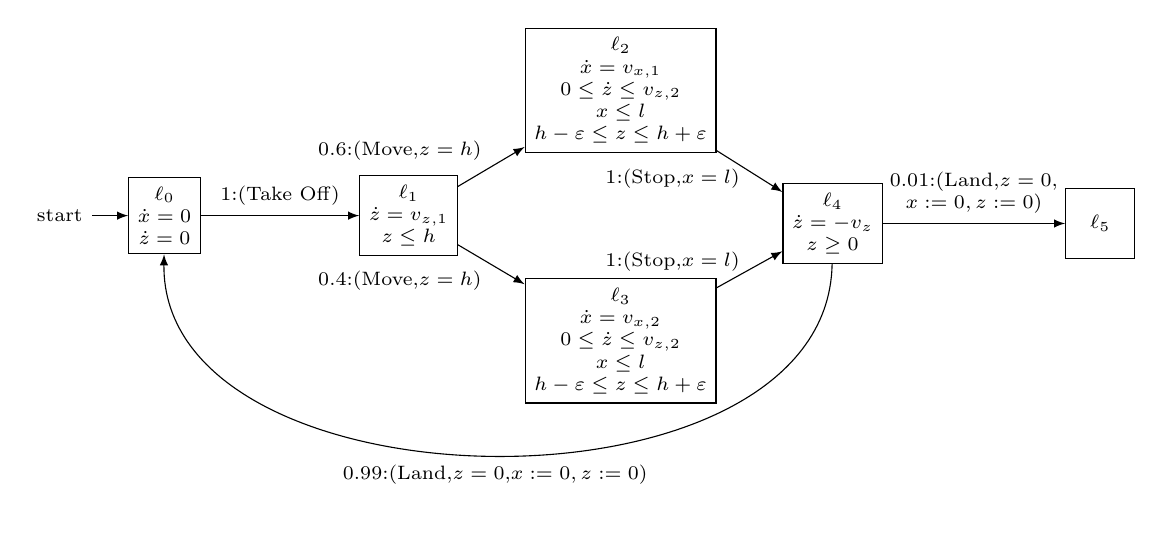
\begin{tikzpicture}[node distance=3.1cm, every state/.style={rectangle}]
             \node [initial, state] (s0) {$\ell_{0}$\\$\dot{x}=0$\\$\dot{z}=0$};
             \node [state] (s1) [right of=s0] {$\ell_{1}$\\$\dot{z}=v_{z,1}$\\$z\leq h$};
             \node [state] (s2) [above right of=s1,yshift=-6mm,xshift=5mm] {$\ell_{2}$\\$\dot{x}=v_{x,1}$\\$0\leq\dot{z}\leq v_{z,2}$\\$x\leq l$\\$h-\varepsilon\leq z\leq h+\varepsilon$};
             \node [state] (s3) [below right of=s1,yshift=6mm,xshift=5mm] {$\ell_{3}$\\$\dot{x}=v_{x,2}$\\$0\leq\dot{z}\leq v_{z,2}$\\$x\leq l$\\$h-\varepsilon\leq z\leq h+\varepsilon$};
             \node [state] (s4) [below right of=s2,yshift=5mm,xshift=5mm] {$\ell_{4}$\\$\dot{z}=-v_{z}$\\$z\geq 0$};
             \node [state] (s5) [right of=s4,xshift=3mm] {$\ell_{5}$};

             \path[->] (s0) edge node [above] {1:(Take Off)} (s1)
                (s1) edge node [left,yshift=2mm] {0.6:(Move,$z=h$)} (s2)
                    edge node [left,yshift=-2mm] {0.4:(Move,$z=h$)} (s3)
                (s2) edge node [left,yshift=-1mm] {1:(Stop,$x=l$)} (s4)
                (s3) edge node [left,yshift=1mm] {1:(Stop,$x=l$)} (s4)
                (s4) edge node [above] {0.01:(Land,$z=0$,\\$x:=0,z:=0$)} (s5)
                    edge [bend left=90] node [below] {0.99:(Land,$z=0$,$x:=0,z:=0$)} (s0);
         \end{tikzpicture}
         \caption{Running example of a UAV.}
         \label{fig:runex}
     \end{center}
 \end{figure}
The different component of the model in Figure~\ref{fig:runex} are
\begin{align*}
    V & = \{x,z\} \\
    L & = \{\ell_{0},\ell_{1},\ell_{2},\ell_{3},\ell_{4},\ell_{5}\} \\
    A & = \{\text{Take Off, Move, Stop, Land}\} \\
    \Init & = \{(\ell_{0},(0,0))\} \\
    \Inv(\ell_{0}) & = \Inv(\ell_{5}) = (\mathbb{R},\mathbb{R})\\
    \Inv(\ell_{1}) & = (\mathbb{R},(-\infty,h])\\
    \Inv(\ell_{2}) & = \Inv(\ell_{3}) = ((-\infty,l],[h-\varepsilon,h+\varepsilon])\\
    \Inv(\ell_{4}) & = (\mathbb{R},[0,\infty))\\
    E & = \{e_{0}=(\ell_{0},\text{Take Off},\ell_{1}), e_{1}=(\ell_{1},\text{Move},\ell_{2}), e_{2}=(\ell_{1},\text{Move},\ell_{3}), & \\
    & e_{3}=(\ell_{2},\text{Stop},\ell_{4}), e_{4}=(\ell_{3},\text{Stop},\ell_{4}), e_{5}=(\ell_{4},\text{Land},\ell_{5}), e_{6}=(\ell_{4},\text{Land},\ell_{5}) \} \\
    r(e_{0}) & = r(e_{1}) = r(e_{2}) = r(e_{3}) = r(e_{4}) = (\mathbb{R},\mathbb{R}) \\
    r(e_{5}) & = r(e_{6}) = (0,0) \\
    g(e_{0}) & = (\mathbb{R},\mathbb{R}) \\
    g(e_{1}) & = g(e_{2}) = (\mathbb{R},h) \\
    g(e_{3}) & = g(e_{4}) = (l,\mathbb{R}) \\
    g(e_{5}) & = g(e_{6}) = (\mathbb{R},0) \\
    f(\ell_{0}) & = f(\ell_{5}) = \{\dot{x} = 0,\dot{z} = 0 \} \\
    f(\ell_{1}) & = \{\dot{x} = 0,\dot{z} = v_{z,1}\} \\
    f(\ell_{2}) & = \{\dot{x} = v_{x,1},\dot{z} = [0,v_{z,2}]\} \\
    f(\ell_{3}) & = \{\dot{x} = v_{x,2},\dot{z} = [0,v_{z,2}]\} \\
    f(\ell_{4}) & = \{\dot{x} = 0,\dot{z}=-v_{z,1}\} \\
    t(\ell_{0},\text{Take Off}) & = \{1: \ell_{1}\} \\
    t(\ell_{1},\text{Move}) & = \{0.6: \ell_{2}, 0.4: \ell_{3}\} \\
    t(\ell_{2},\text{Stop}) & = t(\ell_{3},\text{Stop}) = \{1: \ell_{4}\} \\
    t(\ell_{4},\text{Land}) & = \{0.99: \ell_{0}, 0.01:\ell_{5}\}
\end{align*}
\end{ex}
%\subsection{Abstracting (discrete) Probabilistic Timed Automata}



\subsection{Translating between Different Types of Probabilistic Hybrid Automata}
\label{sec:phatrans}
We can translate between different types of PHAs to reach a PTA which we know can be verified.
The chain of translations goes rectangular to multisingular to stopwatch to timed. Further details on these translations can be found in \cite{Sproston2001}.

In Section~\ref{sec:dpta} we mentioned different ways which are used to verify a PTA.
Using these translations, we can turn the given type of PHA to a PTA, which then can be verified. Note that the PHA has to be initialised to be able to apply the abstraction. This means that the set of initial states contains a single element. Our running example (Example~\ref{ex:abs}) is initialised.

%%%%%%%%%%%%%%%%%%%%%%%%%%%%%%%%%%%%%%%%%%%%%%%%%%%%%%%%%%%%%%%%%%%%%%%%%%%%%%%%%%%%%%%%%%%%%%%%%%%
%%%%%%%%%%%%%%%%%%%%%%%%%%%%%%%%%%%%%%%%%%%%%%%%%%%%%%%%%%%%%%%%%%%%%%%%%%%%%%%%%%%%%%%%%%%%%%%%%%%
%%% PRHA to PMSHA
%%%%%%%%%%%%%%%%%%%%%%%%%%%%%%%%%%%%%%%%%%%%%%%%%%%%%%%%%%%%%%%%%%%%%%%%%%%%%%%%%%%%%%%%%%%%%%%%%%%
%%%%%%%%%%%%%%%%%%%%%%%%%%%%%%%%%%%%%%%%%%%%%%%%%%%%%%%%%%%%%%%%%%%%%%%%%%%%%%%%%%%%%%%%%%%%%%%%%%%
\subsubsection{Rectangular to Multisingular}
The translation from a rectangular to a multisingular PHA is dependent on the maximal and minimal behaviour of the continuous variables, as we are turning the intervals of the flow functions into points. For that new continuous variables are introduced in the multisingular PHA, which represent the extremal flow behaviour, and all conditions in the PHA are adjusted accordingly.

Let $\mathcal{R} = (V_{R},L,A,\Init_{R},\Inv_{R},E_{R},f_{R},t_{R})$ and $\mathcal{M} = (V_{M}, L, A, \Init_{M}, \Inv_{M}, E_{M}, f_{M}, t_{M})$ be a rectangular and a multisingular PHA respectively. We can construct $\mathcal{M}$ from $\mathcal{R}$ by the following steps
\begin{description}
    \item[Continuous Variables] Let $V_{R}=\{x_{1},\ldots,x_{n}\}$ and $V_{M}=\{y_{1},\ldots,y_{2n}\}$ where the $l(i)$-th variable $y_{l(i)}$ represents the lower bound of $x_{i}$ and $y_{u(i)}$ is the upper bound of $x_{i}$, and $l(i)=2i-1,\ u(i)=2i$.

    \item[Initial States] For each $\ell\in L$ let $\Init_{M}(\ell)(y_{l(i)})=\Init_{M}(\ell)(y_{u(i)})=\Init_{R}(\ell)(x_{i})$.

    \item[Invariant Conditions] For each $\ell\in L$ and each $x_{i}\in V_{R}$ if $\Inv_{R}(\ell)(x_{i})=[l,u]$ then
    \begin{align*}
    \Inv_{M}(\ell)(y_{l(i)}) & = [l,\infty), \\
    \Inv_{M}(\ell)(y_{u(i)}) & = (-\infty,u].
    \end{align*}
    \item[Flow] For each $\ell\in L$ and $x_{i}\in V_{R}$ if $f_{R}(\ell)=\dot{x}_{i}\in[l,u]$ then $f_{M}(\ell)(y_{l(i)})= \dot{y}_{l(i)}\in[l,l]$ and $f_{M}(\ell)(y_{u(i)}) = \dot{y}_{u(i)}\in[u,u]$.

    \item[Edges] For each $\ell\in L$, $a\in A$ and $p\in t(\ell,a)$ we can derive a set of edges and distributions in $\mathcal{M}$. To uniquely identify each distribution we have to keep track of status of the reset and guard conditions in $\mathcal{R}$.
    We will assign a \emph{status} number $\{1,\ldots,4\}$ to each variable $x_{i}$ in $\mathcal{R}$ as follows, let $x_{i}$ have bounds $y_{l(i)}$ and $y_{u(i)}$, and let $[gl_{i},gu_{i}]\in g_{R}(e)(x_{i})$, for $e=(\ell,a,\ell')\in E_{R}$ then
    \begin{enumerate}
        \item $\stat(x_{i})=1$ if $y_{l(i)} < gl_{i}$ and $y_{u(i)} \leq gu_{i}$;
        \item $\stat(x_{i})=2$ if $y_{l(i)} < gl_{i}$ and $y_{u(i)} > gu_{i}$;
        \item $\stat(x_{i})=3$ if $y_{l(i)} \geq gl_{i}$ and $y_{u(i)} \leq gu_{i}$;
        \item $\stat(x_{i})=4$ if $y_{l(i)} \geq gl_{i}$ and $y_{u(i)} > gu_{i}$.
    \end{enumerate}
    We can now identify the reset conditions for $\mathcal{M}$ and mark them with the status. Let $e=(\ell,a,\ell')\in E_{R}$ with $r_{R}(e)$ and $g_{R}(e)$ being the reset and guard conditions. Let $x_{i}\in[l_{i},u_{i}]\in g_{R}(e)$ and should $x_{i}$ be
    reset on $e$ then it will be of the form $x_{i}\in[l_{i}',u_{i}']\in r_{R}(e)$.
    \begin{itemize}
        \item If $x_{i}$ is reset then $y_{l(i)}=l_{i}'\in r_{M}^{st}(e)$ and $y_{u(i)}=u_{i}'\in r_{M}^{st}(e)$ for each $st\in\{1,\ldots,4\}$.
        \item If $x_{i}$ is not reset then
            \begin{itemize}
                \item if $\stat(x_{i})=1$ then $y_{l(i)}=l_{i}\in r_{M}^{1}(e)$ and $y_{u(i)}\notin r_{M}^{1}(e)$;
                \item if $\stat(x_{i})=2$ then $y_{l(i)}=l_{i}\in r_{M}^{2}(e)$ and $y_{u(i)}=u_{i}\in r_{M}^{2}(e)$;
                \item if $\stat(x_{i})=3$ then $y_{l(i)}\notin r_{M}^{3}(e)$ and $y_{u(i)}\notin r_{M}^{3}(e)$;
                \item if $\stat(x_{i})=4$ then $y_{l(i)}\notin r_{M}^{4}(e)$ and $y_{u(i)}=u_{i}\in r_{M}^{4}(e)$.
            \end{itemize}
    \end{itemize}
    We utilise a similar system to establish the guard conditions in $\mathcal{M}$. For every $x_{i}\in V_{R}$, if $x_{i}\in[l,u]\in g_{R}(e)$ then
        \begin{itemize}
            \item if $\stat(x_{i})=1$ then $y_{l(i)}\in(-\infty,l)\in g_{M}^{1}(e)$ and $y_{u(i)}\in[l,u]\in g_{M}^{1}(e)$;
            \item if $\stat(x_{i})=2$ then $y_{l(i)}\in(-\infty,l)\in g_{M}^{2}(e)$ and $y_{u(i)}\in(u,\infty)\in g_{M}^{2}(e)$;
            \item if $\stat(x_{i})=3$ then $y_{l(i)}\in[l,u]\in g_{M}^{3}(e)$ and $y_{u(i)}\in[l,u]\in g_{M}^{3}(e)$;
            \item if $\stat(x_{i})=4$ then $y_{l(i)}\in[l,u]\in g_{M}^{4}(e)$ and $y_{u(i)}\in(u,\infty)\in g_{M}^{4}(e)$.
        \end{itemize}

    \item[Probabilistic Transition] Through the classification of the guard and reset conditions we can now calculate the probabilistic transitions. We say that we obtain $e=(\ell,a,\ell')\in E_{M}$ with $g_{M}^{st}(e_{M})$ and $r_{M}^{st}(e_{M})$ from $e=(\ell,a,\ell')\in E_{R}$ with $g_{R}(e_{R})$ and $r_{R}(e_{R})$, and denote this by $e\leadsto e^{st}$, then
    \[
    t_{M}^{st}(\ell,a)(\ell') = \sum_{\substack{t_{R}(\ell,a)(\ell')\neq0 \land\\ e\leadsto e^{st}}} t_{R}(\ell,a)(\ell')
    \]
    for each $st\in\{1,\ldots,4\}$.
\end{description}



\begin{ex}
    \label{ex:rect2ms}
Take the rectangular hybrid automaton defined in Example~\ref{ex:abs}. Using the above description we can translate that hybrid automaton to a multisingular hybrid automaton $\mathcal{M}=(V,L,A,\Init,\Inv,E,f,t)$ where the components are
\begin{itemize}
    \item $V=\{x_{l},x_{u},z_{l},z_{u}\}$
    \item $L=\{\ell_{0},\ell_{1},\ell_{2},\ell_{3},\ell_{4},\ell_{5}\}$
    \item $A=\{\text{TakeOff, Move, Stop, Land}\}$
    \item $\Init=\{(\ell_{0},(0,0,0,0))\}$
    \item The invariant conditions are
    \begin{align*}\Inv(\ell_{0})=&\Inv(\ell_{5})=(\mathbb{R},\mathbb{R},\mathbb{R},\mathbb{R})\\
        \Inv(\ell_{1})=&(\mathbb{R},\mathbb{R},\mathbb{R},(-\infty,h]), \\
        \Inv(\ell_{2})=&\Inv(\ell_{3})=(\mathbb{R},(-\infty,l],[h-\varepsilon,\infty),(-\infty,h+\varepsilon]), \\
        \Inv(\ell_{4})=& (\mathbb{R},\mathbb{R},[0,\infty),\mathbb{R})
    \end{align*}
    \item The flow conditions are
    \begin{align*}
        f(\ell_{0})=&f(\ell_{5})=\{\dot{x}_{l}=\dot{x}_u=\dot{z}_{l}=\dot{z}_{u}=0\},\\
        f(\ell_{1})=&\{\dot{x}_{l}=\dot{x}_{u}=0,\dot{z}_{l}=\dot{z}_{u}=v_{z1}\},\\
        f(\ell_{2})=&\{\dot{x}_{l}=\dot{x}_{u}=v_{x1},\dot{z}_{l}=0,\dot{z}_{u}=v_{z2}\},\\
        f(\ell_{3})=&\{\dot{x}_{l}=\dot{x}_{u}=v_{x2},\dot{z}_{l}=0,\dot{z}_{u}=v_{z2}\},\\
        f(\ell_{4})=&\{\dot{x}_{l}=\dot{x}_{u}=0,\dot{z}_{l}=\dot{z}_{u}=-v_{z1}\}
    \end{align*}
    \item The edges, reset conditions, guard conditions and probability distributions are as follows
    \begin{itemize}
        \item The edge $e_{0}=(\ell_{0},)(\text{TakeOff}, \ell_{1})$ from the original hybrid automaton is the same in $\mathcal{M}$ due to its trivial guard and reset conditions for all variables and its Dirac distribution.
        Thus in $\mathcal{M}$, $g(e_{0})=(\mathbb{R},\mathbb{R},\mathbb{R},\mathbb{R})$, $r(e_{0})=\emptyset$ and $t(\ell_{0},)(\text{TakeOff})=\{1:\ell_{1}\}$.
        \item For $(\ell_{1},\text{Move})$ we find that $\stat(x)=3$ and similarily $\stat(z)=3$, the guard and reset conditions for $x_{l},x_{u}$ are trivially induced. Then as $z$ is not reset, $z_{l}$ and $z_{u}$ will not either, and finally as $\stat(z)=3$ the guard conditions are $z_{l}=h$ and $z_{u}=h$.
        Thus $g(\ell_{1},\text{Move},\ell_{2})=g(\ell_{1},\text{Move},\ell_{3})=(\mathbb{R},\mathbb{R},h,h)$ and $r(\ell_{1},\text{Move},\ell_{2})=r(\ell_{1},\text{Move},\ell_{3})=\emptyset$.
        Based on that the probability transition function stays the same for $t(\ell_{1},\text{Move})=\{0.6:\ell_{2},0.4:\ell_{3}\}$.
        \item $(\ell_{2},\text{Stop})$ is transformed similarly as the last edge, with $\stat(x)=\stat(z)=3$. So $g(\ell_{2},\text{Stop},\ell_{4})=(l,l,\mathbb{R},\mathbb{R})$ and $r(\ell_{2},\text{Stop},\ell_{4})=\emptyset$, and $t(\ell_{2},\text{Stop})=\{1:\ell_{4}\}$.
        \item $(\ell_{3},\text{Stop})$ is translated as $(\ell_{2},\text{Stop})$, thus
        $g(\ell_{3},\text{Stop},\ell_{4})=(l,l,\mathbb{R},\mathbb{R})$ and $r(\ell_{3},\text{Stop},\ell_{4})=\emptyset$, and $t(\ell_{3},\text{Stop})=\{1:\ell_{4}\}$.
        \item For $(\ell_{4},\text{Land})$ is translated through $\stat(x)=\stat(z)=3$ thus the reset maps are $r(\ell_{4},\text{Land},\ell_{0})=r(\ell_{4},\text{Land},\ell_{5})=(0,0,0,0)$ and the guard conditions are $g(\ell_{4},\text{Land},\ell_{0})=g(\ell_{4},\text{Land},\ell_{5})=(\mathbb{R},\mathbb{R},0,0)$ and the probability transition function is $t(\ell_{4},\text{Land})=\{0.99:\ell_{0},0.01:\ell_{5}\}$.
    \end{itemize}
\end{itemize}

\end{ex}
%%%%%%%%%%%%%%%%%%%%%%%%%%%%%%%%%%%%%%%%%%%%%%%%%%%%%%%%%%%%%%%%%%%%%%%%%%%%%%%%%%%%%%%%%%%%%%%%%%%
%%%%%%%%%%%%%%%%%%%%%%%%%%%%%%%%%%%%%%%%%%%%%%%%%%%%%%%%%%%%%%%%%%%%%%%%%%%%%%%%%%%%%%%%%%%%%%%%%%%
%%% PMSHA to PSWA
%%%%%%%%%%%%%%%%%%%%%%%%%%%%%%%%%%%%%%%%%%%%%%%%%%%%%%%%%%%%%%%%%%%%%%%%%%%%%%%%%%%%%%%%%%%%%%%%%%%
%%%%%%%%%%%%%%%%%%%%%%%%%%%%%%%%%%%%%%%%%%%%%%%%%%%%%%%%%%%%%%%%%%%%%%%%%%%%%%%%%%%%%%%%%%%%%%%%%%%
\subsubsection{Multisingular To Stopwatch}
From a multisingular PHA $\mathcal{M} = (V,L,A,\Init_{M},\Inv_{M},E,f_{M},t)$ we are going to construct a probabilistic stopwatch automaton $\mathcal{W} = (V,L,A,\Init_{W},\Inv_{W},E,f_{W},t)$. For this abstraction to work, we need to introduce a scaling factor for each variable at each location.

\begin{defi}[Scaling Factor]
    In $\mathcal{M}$ for all $\ell\in L$, $x_{i}\in V$ of $\mathcal{M}$ if $f_{M}(\ell)=\dot{x}\in[k,k]$ for some $k\in\mathbb{Z}$ then the \emph{scaling factor} of $x_{i}$ in $\ell$ is $k_{i}^{\ell}$, where $k_{i}^{\ell}=k$ if $k\neq0$ and $k_{i}^{\ell}=1$ if $k=0$.
\end{defi}
The scaling factor will help with skewing the flow functions to represent clocks (have flow equal to $1$). The construction of $\mathcal{W}$ is done as follows
\begin{description}
    \item[Initial States] Let $\ell\in L$ such that $\Init_{M}(\ell)\neq\emptyset$, and $\Init_{M}(\ell)\in\mathbb{Z}^{n}$. For every $x_{i}\in V$ if $x_{i}\in[k,k]\in \Init_{M}(\ell)$ for some $k\in\mathcal{Z}$ then let
    $x_{i}\in[\frac{k}{k_{i}^{\ell}},\frac{k}{k_{i}^{\ell}}]\in \Init_{W}(\ell)$.
    \item[Invariant Conditions] For each $\ell\in L$ and each $x_{i}\in V$ if the lower and upper bounds of $x_{i}$ in $\Inv_{M}(\ell)$ are $k_{1},k_{2}\in\mathbb{Z}$ respectively, then the lower and upper bounds of $x_{i}$ in $\Inv_{W}(\ell)$ are
    $\frac{k_{1}}{k_{i}^{\ell}},\frac{k_{2}}{k_{i}^{\ell}}$ respectively, and the limits of the interval are the same (open is mapped to open and closed is mapped to closed).
    \item[Flow] For all $\ell\in L$ and all $x_{i}\in V$ if $f_{M}(\ell)=\dot{x}_{i}\in[0,0]$ then $f_{W}(\ell)=\dot{x}_{i}\in[0,0]$ else $f_{W}(\ell)=\dot{x}_{i}\in[1,1]$.
    \item[Edge Conditions] While the edge set is the same in both automata, we need to rescale the reset and guard conditions. Let $e=(\ell,a,\ell')\in E$, then the reset conditions are derived from $r_{M}(e)(x_{i})=k\in\mathbb{Z}$ then $r_{W}(e)(x_{i})= \frac{k}{k_{i}^{\ell'}}$, for each $x_{i}\in V$. The guard conditions are scaled similarly as the invariant conditions, namely for each $x_{i}\in V$ if the lower and upper bounds of
    $x_{i}$ in $g_{M}(e)$ are $k_{1},k_{2}\in\mathbb{Z}$ respectively, then the lower and upper bounds of $x_{i}$ in $g_{W}(e)$ are $\frac{k_{1}}{k_{i}^{\ell}},\frac{k_{2}}{k_{i}^{\ell}}$ respectively, and the limits of the interval are the same (open is mapped to open and closed is mapped to closed).
\end{description}

Note that for this translation to work, the following restriction has to be added to the invariant conditions of the multisingular PHA $\mathcal{M}$. At any location $\ell\in L$ any variable with positive (negative) slope has a finite lower (upper) bound in the invariant. This restriction can be enforced without loss of generality by replacing infinite bounds with the minimal and maximal values the variable can achieve globally \cite{Olivero1994}.

\begin{defi}[[Equivalence between $\mathcal{W}$ and $\mathcal{M}$ \cite{Henzinger1995}]
Let $\mathcal{M}$ be an initialised multisingular PHA, let $\mathcal{W}$ be an initialised probabilistic stopwatch automaton derived from $\mathcal{M}$ as described above, let
 $\mathcal{P}_{M}=(Q^{M},Q^{M}_{0},A^{M},t^{M})$ and
 $\mathcal{P}_{W}=(Q^{W},Q^{W}_{0},A^{W},t^{W})$ be their probabilistic transitions systems (see Definition~\ref{def:pha2pts}) and let $\{k_{i}^{\ell}\in\mathbb{Z} : \ell\in L_{M}, x_{i}\in X\}$ be the set of scaling factors of $\mathcal{M}$. Then let $\sigma : Q^{W} \rightarrow Q^{M}$ be the
 bijection such that for each $(\ell, \val(x))\in Q^{W}$ we have $\sigma(\ell,\val(x))=(\ell,\val(y))$ where $\val(y)_{i} = k_{i}^{\ell}\val(x)_{i}$ for each $x_{i}\in X$.
 The relation $\sim_{\sigma}$ is an equivalence on $Q^{W}\cup Q^{M}$ such that $s\sim_{\sigma}s'$ if and only if $\sigma(s)=s'$ for $s\in Q^{M}$ and $s'\in Q^{W}$.
\end{defi}

\begin{prop}[\cite{Sproston2001}]
Let $\mathcal{M}$ be an initialised multisingular PHA and let $\mathcal{W}$ be the initialised stopwatch automaton constructed from $\mathcal{M}$ using the method described above. Then the equivalence relation $\sim_{\sigma}$ is a bisimulation between $\mathcal{P}_{M}$ and $\mathcal{P}_{W}$.
\end{prop}


\begin{ex}
\label{ex:ms2sw}
We are going to translate the resulting automaton from Example~\ref{ex:rect2ms} into a probabilistic stopwatch automaton. For that we need to restrict the invariant conditions of our multisingular hybrid automaton to
\begin{align*}
    \Inv(\ell_{0})=&\Inv(\ell_{5})=(\mathbb{R},\mathbb{R},\mathbb{R},\mathbb{R})\\
    \Inv(\ell_{1})=&(\mathbb{R},\mathbb{R},[0,\infty),[0,h]), \\
    \Inv(\ell_{2})=&\Inv(\ell_{3})=([0,\infty),[0,l],[h-\varepsilon,\infty),[0,h+\varepsilon]), \\
    \Inv(\ell_{4})=& (\mathbb{R},\mathbb{R},[0,h+\varepsilon],(-\infty,h+\varepsilon]).
\end{align*}

Further we need to calculate the scaling factors of the continuous variables in each location, see Table~\ref{tab:sf}. Now we can utilise these factors to construct a probabilistic stopwatch automaton from the multisingular probabilistic hybrid automaton in Example~\ref{ex:rect2ms} (with adjusted invariant conditions).
\begin{table}
\begin{center}
    \begin{tabular}{c|c|c|c|c|c|c}
                & $\ell_{0}$ & $\ell_{1}$ & $\ell_{2}$ & $\ell_{3}$ & $\ell_{4}$ & $\ell_{5}$ \\ \hline
        $x_{l}$ & $1$ & $1$ & $v_{x1}$ & $v_{x2}$ & $1$ & $1$ \\ \hline
        $x_{u}$ & $1$ & $1$ & $v_{x1}$ & $v_{x2}$ & $1$ & $1$ \\ \hline
        $z_{l}$ & $1$ & $v_{z1}$ & $1$ & $1$ & $-v_{z1}$ & $1$ \\ \hline
        $z_{u}$ & $1$ & $v_{z1}$ & $v_{z2}$ & $v_{z2}$ & $-v_{z1}$ & $1$

    \end{tabular}
    \caption{Table of scaling factors for translation of the running example.}
    \label{tab:sf}
\end{center}
\end{table}
\begin{itemize}
    \item $V=\{x_{l},x_{u},z_{l},z_{u}\}$
    \item $L=\{\ell_{0},\ell_{1},\ell_{2},\ell_{3},\ell_{4},\ell_{5}\}$
    \item $A=\{\text{TakeOff, Move, Stop, Land}\}$
    \item $\Init=\{(\ell_{0},(0,0,0,0))\}$
    \item The invariants for the locations are as above stated
     \begin{align*}
        \Inv(\ell_{0})=&\Inv(\ell_{5})=(\mathbb{R},\mathbb{R},\mathbb{R},\mathbb{R})\\
        \Inv(\ell_{1})=&(\mathbb{R},\mathbb{R},[0,\infty),[0,\frac{h}{v_{z1}}]), \\
        \Inv(\ell_{2})=&([0,\infty),[0,\frac{l}{v_{x1}}],[h-\varepsilon,\infty),[0,\frac{h+\varepsilon}{v_{z2}}]), \\
        \Inv(\ell_{3})=&([0,\infty),[0,\frac{l}{v_{x2}}],[h-\varepsilon,\infty),[0,\frac{h+\varepsilon}{v_{z2}}]), \\
        \Inv(\ell_{4})=&(\mathbb{R},\mathbb{R},[-\frac{h+\varepsilon}{v_{z1}},0],[-\frac{h+\varepsilon}{v_{z1}},\infty))
    \end{align*}
    \item $E=\{e_{0}=(\ell_{0},\text{TakeOff},\ell_{1}), e_{1}=(\ell_{1},\text{Move},\ell_{2}), e_{2}=(\ell_{1},\text{Move},\ell_{3}), e_{3}=(\ell_{2},\text{Stop},\ell_{4}), e_{4}=(\ell_{3},\text{Stop},\ell_{4}), e_{5}=(\ell_{4},\text{Land},\ell_{5}), e_{6}=(\ell_{4},\text{Land},\ell_{0})\}$ is the set of edges, which is the same as in the multisingular automaton before. The guard conditions are defined as
    \begin{align*}
        g(e_{0})= & (\mathbb{R},\mathbb{R},\mathbb{R},\mathbb{R}) \\
        g(e_{1})= & g(e_{2}) = (\mathbb{R},\mathbb{R},\frac{h}{v_{z1}},\frac{h}{v_{z1}}) \\
        g(e_{3})= & (\frac{l}{v_{x1}}, \frac{l}{v_{x1}}, \mathbb{R},\mathbb{R}) \\
        g(e_{4})= & (\frac{l}{v_{x2}}, \frac{l}{v_{x2}}, \mathbb{R},\mathbb{R}) \\
        g(e_{5})= & g(e_{6})=(\mathbb{R},\mathbb{R},0,0),
    \end{align*}
    and the reset maps are
    \begin{align*}
        r(e_{0})= & (x_{l},x_{u},\frac{z_{l}}{v_{z1}},\frac{z_{u}}{v_{z1}})\\
        r(e_{1})= & (\frac{x_{l}}{v_{x1}},\frac{x_{u}}{v_{x1}},z_{l},\frac{z_{u}}{v_{z2}}) \\
        r(e_{2})= & (\frac{x_{l}}{v_{x2}},\frac{x_{u}}{v_{x2}},z_{l},\frac{z_{u}}{v_{z2}}) \\
        r(e_{3})= & r(e_{4})=(x_{l},x_{u},-\frac{z_{l}}{v_{z1}},-\frac{z_{u}}{v_{z1}})\\
        r(e_{5})=& r(e_{6})=(0,0,0,0).
    \end{align*}
    \item We transform the flow conditions to the following
    \begin{align*}
        f(\ell_{0})=f(\ell_{5})=& \{\dot{x}_{l}=\dot{x}_{u}=\dot{z}_{l}=\dot{z}_{u}=0\} \\
        f(\ell_{1})=f(\ell_{4})=& \{\dot{x}_{l}=\dot{x}_{u}=0,\dot{z}_{l}=\dot{z}_{u}=1\} \\
        f(\ell_{2})=f(\ell_{3})=& \{\dot{x}_{l}=\dot{x}_{u}=\dot{z}_{u}=1,\dot{z}_{l}=0\}.
    \end{align*}
    \item The probabilistic transition function is the same as for the multisingular probabilistic hybrid automaton.
\end{itemize}
\end{ex}

%%%%%%%%%%%%%%%%%%%%%%%%%%%%%%%%%%%%%%%%%%%%%%%%%%%%%%%%%%%%%%%%%%%%%%%%%%%%%%%%%%%%%%%%%%%%%%%%%%%
%%%%%%%%%%%%%%%%%%%%%%%%%%%%%%%%%%%%%%%%%%%%%%%%%%%%%%%%%%%%%%%%%%%%%%%%%%%%%%%%%%%%%%%%%%%%%%%%%%%
%%% PSWA to PTA
%%%%%%%%%%%%%%%%%%%%%%%%%%%%%%%%%%%%%%%%%%%%%%%%%%%%%%%%%%%%%%%%%%%%%%%%%%%%%%%%%%%%%%%%%%%%%%%%%%%
%%%%%%%%%%%%%%%%%%%%%%%%%%%%%%%%%%%%%%%%%%%%%%%%%%%%%%%%%%%%%%%%%%%%%%%%%%%%%%%%%%%%%%%%%%%%%%%%%%%
\subsubsection{Stopwatch To Timed}
We will now translate a probabilistic stopwatch automaton $\mathcal{W} = (V,A,\Init_{W},\Inv_{W},E_{W},f_{W},t_{W})$ to a probabilistic timed automaton $\mathcal{T} = (V,A,\Init_{T},\Inv_{T},E_{T},f_{T},t_{T})$. This translation will turn all the remaining flow conditions from 0 to 1. For that we introduce a new variable $\bot$ which represents abstract time, and with that we will extend model, as follows;

\begin{description}
\item[Locations] Let $K$ be the set of integer constants of the guard, reset, initial or invariant  conditions of $\mathcal{W}$, let $K_{\bot}=K\cup\{\bot\}$. Then $L_{T}=L_{W}\times \Gamma$, where $\Gamma$ is a set of functions of the form $\gamma:V\rightarrow K_{\bot}$. For a given
$\ell\in L_{W}$ the location in $\mathcal{T}$ is of the form $(\ell,\gamma)\in L_{T}$, where for each $x_{i}\in V$ if $f_{W}(\ell)=\dot{x}_{i}=1$ then $\gamma(x_{i}) = \bot$, otherwise
$\gamma(x_{i})\in K$.
\item[Initial States] For all $(\ell,\gamma)\in L_{T}$ if for each $x_{i}\in V$ either $\gamma(x_{i}) = \bot$, or $\gamma(x_{i}) = \Init_{W}(\ell)(x_{i})$ then let $\Init_{T}(\ell,\gamma) = \Init_{W}(\ell)$ otherwise $\Init_{T}(\ell,\gamma)=\emptyset$.
\item[Invariant Conditions] For all $(\ell,\gamma)\in L_{T}$, for each $x_{i}\in V$ if
    \begin{itemize}
        \item $\gamma(x_{i}) = \bot$ then $\Inv_{T}(\ell,\gamma)(x_{i}) = \Inv_{W}(\ell)(x_{i})$.
        \item $\gamma(x_{i}) \in \Inv_{W}(\ell)(x_{i})$ then $\Inv_{T}(\ell,\gamma)(x_{i})=\mathbb{R}_{\geq 0}$
        \item $\gamma(x_{i}) \notin \Inv_{W}(\ell)(x_{i})$ then $\Inv_{T}(\ell,\gamma)(x_{i})=\emptyset$.
    \end{itemize}
\item[Edge Conditions] We derive the edge set for $\mathcal{T}$ as follows, let $e_{W}=(\ell,a,\ell')\in E_{W}$ then there exists $((\ell,\gamma), a, (\ell',\gamma'))\in E_{T}$ where for every $x_{i}\in V$ either
    \begin{itemize}
        \item $f_{W}(\ell')=\dot{x}_{i} = 1$ and $\gamma'(x_{i}) = \bot$
        \item $f_{W}(\ell)=\dot{x}_{i}=1$, $f_{W}(\ell')=\dot{x}_{i}=0$ and $\gamma'(x_{i})=r_{W}(e_{W})(x_{i})$
        \item $f_{W}(\ell)=\dot{x}_{i}=0$, $f_{W}(\ell')=\dot{x}_{i}=0$, $x_{i}$ does not get reset and $\gamma'(x_{i})=\gamma(x_{i})$
        \item $f_{W}(\ell)=\dot{x}_{i}=0$, $f_{W}(\ell')=\dot{x}_{i}=0$, $r_{W}(e_{W})(x_{i})$ exists and $\gamma'(x_{i})=r_{W}(e_{W})(x_{i})$.
    \end{itemize}
The reset maps stay the same, and are distributed onto the new edges accordingly to $\ell'\in L_{W}$. The guard conditions on an edge for a variable $x_{i}$ is the same as in the stopwatch automaton if $\gamma(x_{i})=\bot$, otherwise if $\gamma(x_{i})\in g_{W}(e)$ then let $g_{T}(e)(x_{i})=\mathbb{R}_{\geq 0}$, else $x_{i}$ is unguarded.
\item[Probability transitions] Let $t_{W}(\ell,a) = \{p_{W}^{1},\ldots,p_{W}^{l}\}$ be the probabilities from $\ell\in L_{W}$, and $t_{T}((\ell,\gamma),a) = \{p_{T}^{1},\ldots,p_{T}^{l}\}$.
Then for each $\ell'\in L_{W}$ in $(\ell,a,\ell')\in E$ there exists a $(\ell',\gamma)\in L_{T}$ according to the construction of the edges above and then $p_{T}^{j}(\ell',\gamma) = p_{W}^{j}(\ell')$, for $1\leq j \leq l$.
\end{description}

Note that $\bot$ can be seen as a abstract time passing variable.

\begin{defi}[Equivalence between $\mathcal{T}$ and $\mathcal{W}$ \cite{Henzinger1995}]
Let $\mathcal{W}$ be an initialised probabilistic stopwatch automaton, let $\mathcal{T}$ be a probabilistic timed automaton derived from $\mathcal{W}$ as described above, let
$\mathcal{P}_{W}=(Q^{W},Q^{W}_{0},A^{W},t^{W})$ and $\mathcal{P}_{T}=(Q^{T},Q^{T}_{0},A^{T},t^{T})$ be their associated probabilistic transition systems (see Definition~\ref{def:pha2pts}). Then
$\tau : Q^{T}\rightarrow Q^{W}$ is defined such that for each $((\ell,\gamma),\val(v))\in Q^{T}$, we have $\tau((\ell,\gamma),\val(x))=(\ell,\val(y))$ where $\val(x)_{i}=\val(y)_{i}$ if
$\gamma(x_{i})=\bot$ and otherwise $\val(y_{i})=\gamma(x_{i})$, for each $x_{i}\in V$. The relation $\sim_{\tau}$ is an equivalence on $Q^{T}\cup Q^{W}$ such that $q\sim_{\tau}q'$ if and only if  $\tau(q)=q'$ for $q\in Q^{T}$ and $q'\in Q^{W}$.
\end{defi}

\begin{prop}[\cite{Sproston2001}]
Let $\mathcal{W}$ be an initialised probabilistic stopwatch automaton, and let $\mathcal{T}$ be the probabilistic timed automaton derived from $\mathcal{W}$ using the method above. Then the equivalence $\sim_{\tau}$ is a bisimulation between $\mathcal{P}_{W}$ and $\mathcal{P}_{T}$.
\end{prop}


\begin{ex}
We will now translate the stopwatch automaton resulting in Example~\ref{ex:ms2sw} to a PTA.
\begin{itemize}
    \item First we calculate a preliminary set of locations. We will extend the set once the initial state and edges have been determined.
    \begin{align*}
    L=\{&(\ell_{0},(\gamma(x_{l}),\gamma(x_{u}),\gamma(z_{l}),\gamma(z_{u}))), \\
        &(\ell_{1},(\gamma(x_{l}),\gamma(x_{u}),\bot,\bot)), \\
        &(\ell_{2},(\bot,\bot,\gamma(z_{l}),\bot)), \\
        &(\ell_{3},(\bot,\bot,\gamma(z_{l}),\bot)), \\
        &(\ell_{4},(\gamma(x_{l}),\gamma(x_{u}),\bot,\bot)), \\
        &(\ell_{5},(\gamma(x_{l}),\gamma(x_{u}),\gamma(z_{l}),\gamma(z_{u})))\}
    \end{align*}
    \item $\Init=(\ell_{0},(0,0,0,0))$
    \item We can find the set of edges to be
    \begin{align*}
    E=\{e_{0}=&((\ell_{0},(0,0,0,0)),\text{TakeOff},(\ell_{1},(0,0,\bot,\bot))), \\
        e_{1}=&((\ell_{1},(0,0,\bot,\bot)),\text{Move},(\ell_{2},(\bot,\bot,\frac{h}{v_{z1}}))),\\
        e_{2}=&((\ell_{1},(0,0,\bot,\bot)),\text{Move},(\ell_{3},(\bot,\bot,\frac{h}{v_{z1}}))),\\
        e_{3}=&((\ell_{2},(\bot,\bot,\frac{h}{v_{z1}})),\text{Stop},(\ell_{4},(\frac{l}{v_{x1}},\frac{l}{v_{x1}},\bot,\bot))),\\
        e_{4}=&((\ell_{3},(\bot,\bot,\frac{h}{v_{z1}})),\text{Stop},(\ell_{4},(\frac{l}{v_{x2}},\frac{l}{v_{x2}},\bot,\bot))),\\
        e_{5}=&(\ell_{4},(\frac{l}{v_{x1}},\frac{l}{v_{x1}},\bot,\bot)),\text{Land},(\ell_{5},(0,0,0,0))),\\
        e_{6}=&(\ell_{4},(\frac{l}{v_{x1}},\frac{l}{v_{x1}},\bot,\bot)),\text{Land},(\ell_{0},(0,0,0,0))),\\
        e_{7}=&(\ell_{4},(\frac{l}{v_{x2}},\frac{l}{v_{x2}},\bot,\bot)),\text{Land},(\ell_{5},(0,0,0,0))),\\
        e_{8}=&(\ell_{4},(\frac{l}{v_{x2}},\frac{l}{v_{x2}},\bot,\bot)),\text{Land},(\ell_{0},(0,0,0,0)))\},
    \end{align*}
    then the guard conditions are
    \begin{align*}
        g(e_{0})= & (\mathbb{R},\mathbb{R},\mathbb{R},\mathbb{R}) \\
        g(e_{1})= & g(e_{2}) = (\mathbb{R},\mathbb{R},\frac{h}{v_{z1}},\frac{h}{v_{z1}}) \\
        g(e_{3})= & (\frac{l}{v_{x1}}, \frac{l}{v_{x1}}, \mathbb{R},\mathbb{R}) \\
        g(e_{4})= & (\frac{l}{v_{x2}}, \frac{l}{v_{x2}}, \mathbb{R},\mathbb{R}) \\
        g(e_{5})= & g(e_{6})=g(e_{7})=g(e_{8})=(\mathbb{R},\mathbb{R},0,0),
    \end{align*}
    and the reset maps are
    \begin{align*}
        r(e_{0})=&(x_{l},x_{u},\frac{z_{l}}{v_{z1}},\frac{z_{u}}{v_{z1}})\\
        r(e_{1})=&(\frac{x_{l}}{v_{x1}},\frac{x_{u}}{v_{x1}},z_{l},\frac{z_{u}}{v_{z2}}) \\
        r(e_{2})=&(\frac{x_{l}}{v_{x2}},\frac{x_{u}}{v_{x2}},z_{l},\frac{z_{u}}{v_{z2}}) \\
        r(e_{3})=&r(e_{4})=(x_{l},x_{u},-\frac{z_{l}}{v_{z1}},-\frac{z_{u}}{v_{z1}})\\
        r(e_{5})=&r(e_{6})=r(e_{7})=r(e_{8})=(0,0,0,0).
    \end{align*}
    \item So the set of locations is
    \begin{align*}
        L=\{&(\ell_{0},(0,0,0,0)),(\ell_{1},(0,0,\bot,\bot)),(\ell_{2},(\bot,\bot,\frac{h}{v_{z1}},\bot)),\\
        &(\ell_{3},(\bot,\bot,\frac{h}{v_{z1}},\bot)),(\ell_{4},(\frac{l}{v_{x1}},\frac{l}{v_{x1}},\bot,\bot)),(\ell_{4},(\frac{l}{v_{x2}},\frac{l}{v_{x2}},\bot,\bot)),\\
        &(\ell_{5},(0,0,0,0))\}
    \end{align*}
    \item The invariant conditions for each location are computed to be
    \begin{align*}
            \Inv(\ell_{0},(0,0,0,0))&=\Inv(\ell_{5},(0,0,0,0))=\emptyset \\
            \Inv(\ell_{1},(0,0,\bot,\bot))&=(\mathbb{R}_{\geq0},\mathbb{R}_{\geq0},[0,\infty),[0,\frac{h}{v_{z1}}]) \\
            \Inv(\ell_{2},(\bot,\bot,\frac{h}{v_{z1}},\bot))&=([0,\infty),[0,\frac{l}{v_{x1}}],\mathbb{R}_{\geq0},[0,\frac{h+\varepsilon}{v_{z2}}]) \\
            \Inv(\ell_{3},(\bot,\bot,\frac{h}{v_{z1}},\bot))&=([0,\infty),[0,\frac{l}{v_{x2}}],\mathbb{R}_{\geq0},[0,\frac{h+\varepsilon}{v_{z2}}]) \\
            \Inv(\ell_{4},(\frac{l}{v_{x1}},\frac{l}{v_{x1}},\bot,\bot))&=(\mathbb{R}_{\geq0},\mathbb{R}_{\geq0},[-\frac{h+\varepsilon}{v_{z1}},0],[-\frac{h+\varepsilon}{v_{z1}},0]) \\
            \Inv(\ell_{4},(\frac{l}{v_{x2}},\frac{l}{v_{x2}},\bot,\bot))&=(\mathbb{R}_{\geq0},\mathbb{R}_{\geq0},[-\frac{h+\varepsilon}{v_{z1}},0],[-\frac{h+\varepsilon}{v_{z1}},0])
    \end{align*}
    \item As this resulting automaton is a probabilistic timed automaton, the flow condition in each location, for all variables is $1$.
    \item The probabilistic transition function for each edge is computed to be
    \begin{align*}
        t((\ell_{0},(0,0,0,0)),\text{TakeOff})&=\{1:(\ell_{1},(0,0,\bot,\bot))\} \\
        t((\ell_{1},(0,0,\bot,\bot)),\text{Move})&=\{0.6:(\ell_{2},(\bot,\bot,\frac{h}{v_{z1}},\bot)),0.4:(\ell_{3},(\bot,\bot,\frac{h}{v_{z1}},\bot))\}\\
        t((\ell_{2},(\bot,\bot,\frac{h}{v_{z1}},\bot)),\text{Stop})&=\{1:(\ell_{4},(\frac{l}{v_{x1}},\frac{l}{v_{x1}},\bot,\bot))\} \\
        t((\ell_{3},(\bot,\bot,\frac{h}{v_{z1}},\bot)),\text{Stop})&=\{1:(\ell_{4},(\frac{l}{v_{x2}},\frac{l}{v_{x2}},\bot,\bot))\} \\
        t((\ell_{4},(\frac{l}{v_{x1}},\frac{l}{v_{x1}},\bot,\bot)),\text{Land})&=\{0.99:(\ell_{0},(0,0,0,0)),0.01:(\ell_{5},(0,0,0,0))\} \\
        t((\ell_{4},(\frac{l}{v_{x2}},\frac{l}{v_{x2}},\bot,\bot)),\text{Land})&=\{0.99:(\ell_{0},(0,0,0,0)),0.01:(\ell_{5},(0,0,0,0))\}.
    \end{align*}
\end{itemize}
\end{ex}


\subsection{Abstracting Stochastic Hybrid Automata}
We are now going to look into how a hybrid automaton with stochastic distributions can be abstracted into a probabilistic hybrid automaton. Should the output PHA have the right form we can translate it to a PTA (Section~\ref{sec:phatrans}) and verify the PTA.
Note that we use the notation of SHAs introduced in Section~\ref{sec:sha}.

\begin{defi}[Command Abstraction \cite{Hahn2012}]
Let $c=(g\rightarrow L)$ be a measurable continuous guarded command, choose $p_{i}\geq0$ with $1\leq i\leq n$ and $\sum_{i=1}^{n} p_{i} = 1$. Let
$\hat{u}_{1},\ldots,\hat{u}_{n}:Q\rightarrow \Sigma_{Q}$ and $u_{1},\ldots,u_{n} : Q\rightarrow \Sigma_{Q}$ be functions where $\forall q\in Q$ we have
\begin{itemize}
    \item $\hat{u}_{i}$ and $u_{i}$ are $\Sigma_{Q}-H(\Sigma_{Q})$-measurable $\forall i\in\{1,\ldots,n\}$;
    \item $L(q)(\hat{u}_{i}(q)) = p_{i}$;
    \item $L(q)(\bigcup_{i=1}^{n}\hat{u}_{i}(q)) = 1$;
    \item $\hat{u}_{1}(q),\ldots,\hat{u}_{n}(q)$ are pairwise disjoint;
    \item $\hat{u}_{i}(q)\subseteq u_{i}(q)$ $\forall i\in\{1,\ldots,\}$.
\end{itemize}
A \emph{command abstraction} is $\mathbf{f}=(\hat{u}_{1},\ldots,\hat{u}_{n},u_{1},\ldots,u_{n},p_{1},\ldots,p_{n})$ and the measurable finite guarded command is defined as $abs(c,\mathbf{f}) = (g\rightarrow p_{1}:u_{1}+\cdots+p_{n}:u_{n})$.
\end{defi}

To abstract the SHA into a LTS we first abstract it into a PHA, before abstracting that PHA to an PTA using the translations described in Section~\ref{sec:phatrans}. Note that the PHA here has (on first sight) different components to our earlier definition, this is just because some of the components are hidden within the definitions, or within other component, for example $\Inv$ is contained within the definition of the flow function $f$. Extracting these components is trivial, and shown in the example below.

\begin{defi}[SHA to PHA Abstraction \cite{Hahn2012}]
Let $\mathcal{S}=(V,L,\Init,f,\tfin,\tcont)$ be a SHA and $\mathbf{F}=\langle\mathbf{f}_{c}\rangle_{c\in \tcont}$ a family of command abstractions. Then the \emph{PHA abstraction of $\mathcal{S}$} is $abs(\mathcal{S},\mathbf{F})=(V,L,\Init,f,t)$ defined as follows
\begin{itemize}
    \item $V$, $L$, $\Init$ and $f$ are inherited from $\mathcal{S}$;
    \item $t$ is defined as the disjoint union of $\tfin\cup\{abs(c,\mathbf{f}_{c}) : c \in \tcont\}$.
\end{itemize}
\end{defi}


% \begin{defi}[Abstract State Space]
% An \emph{abstract state space} of a state space $Q=L\times \val(V)$ is a finite set $Q_{A} = \{ q_{1},\ldots,q_{n}\}\subseteq L\times 2^{\val(V)}$ where $q=(\ell,\theta)\in Q_{A}$ and we have $\bigcup_{(\ell,\theta)\in Q} \theta = \val(V)$ for all $\ell\in L$.
% \end{defi}
%
% \begin{rem}
%     $Q_{A}$ does not necessary need to be a partitioning of $L\times\val(V)$.
% \end{rem}
%
% \begin{defi}[Time Restriction]
% A \emph{time restriction} $\mathbf{T}=\langle \mathbf{t}_{\ell}\rangle_{\ell\in L}$ for $f$  is defined such that for each $\ell\in L$ we have
% \begin{itemize}
%     \item $\mathbf{t}_{\ell} : \val(V)\rightarrow \mathbb{R}_{\geq0}$
%     \item for each $v\in\val(V)$, $\mathbf{t}\geq0$ and $v'\in f(\ell)(v)(\mathbf{t})$ there is $n\geq1$ for which there are $v_{1}\ldots,v_{n}\in\val(V)$ and
%     $\mathbf{t}_{1},\ldots,\mathbf{t}_{n-1}\in\mathbb{R}_{\geq0}$ where
%         \begin{itemize}
%             \item $v=v_{1}$
%             \item $v'=v_{n}$
%             \item $\sum_{i} \mathbf{t}_{i} = \mathbf{t}$
%             \item for $i$ with $1\leq i\leq n$ we have $\mathbf{t}_{i}\leq \mathbf{t}_{\ell}(v_{i})$ and $v_{i+1}\in \Inv(\ell)$.
%         \end{itemize}
% \end{itemize}
% \end{defi}
%
% \begin{defi}[Lifted Distribution]
% Let $Q_{A}$ be an abstract state space and $p=[q_{1}\mapsto p_{1},\ldots,q_{n}\mapsto p_{n}]\in\mu(Q)$. The set of \emph{lifted distributions} is defined as
% \[
% Lift_{Q_{A}}(p) = \{[a_{1}\mapsto p_{1},\ldots,a_{n}\mapsto p_{n} : a_{1},\ldots,a_{n}\in Q_{A} \text{ and } q_{1}\in a_{1},\ldots, q_{n}\in a_{n}\}.
% \]
% \end{defi}
%
% \begin{rem}
% If $Q_{A}$ is a partitioning of $L\times \val(V)$ then $Lift_{Q_{A}}$ is a singleton.
% \end{rem}
%
% \begin{defi}[PHA to LTS Abstraction \cite{Hahn2012}]
% \label{def:phs2lts}
% Let $abs(\mathcal{S},\mathbf{F})=(V,L,\Init,f,t_{H})$ be a PHA abstraction of a SHA, $Q_{A}$ an abstract state space, and $\mathbf{T}$ a time restriction, then $\mathcal{P}=(Q,Q_{0},A,t_{P})$ is an \emph{abstraction} of $\mathcal{P}$ using $Q_{A}$ and $\mathbf{T}$ if
% \begin{itemize}
%     \item $Q=Q_{A}$
%     \item $(\Init,0,\ldots,0)\in Q_{0}$
%     \item $A=t_{H}\cup{\bot}$,
%     \item $\forall s\in Q_{A}$ and $q\in s$, $c=(g\rightarrow p_{1}:u_{1}+\cdots+p_{n}:u_{n})\in t_{H}$, if $q\in s\cap g$ then for all $p\in\{[s'_{1}\mapsto p_{1},\ldots,s'_{n}\mapsto p_{n}] : s'_{1}\in u_{1}(s),\ldots, s'_{n}\in u_{n}(s)\}$ there is $p_{A}\in Lift_{Q_{A}}(p)$ with $p_{A}\in t_{P}(s,c)$.
%     \item $\forall q\in Q_{A}$, $s=(\ell,v)\in q$, $\delta\in\mathbb{R}_{\geq 0}$ with $\delta\leq \mathbf{t}_{\ell}(v)$ and all $s'=(\ell,v')\in f(\ell)(s)(\delta)$ if $s'\notin q$ then there is $q'\in Q_{A}$ with $s'\in q'$ and $[q'\mapsto 1]\in t_{P}(q,\bot)$
% \end{itemize}
% \end{defi}
%
% \begin{rem}
% By $\bot$ we denote the single action that some time has passed.
% \end{rem}


\begin{ex}
For the stochastic hybrid automata we have to use a different example to illustrate the abstraction technique above.
In this example we have a UAV flying forward for a given distance, it might find an object on the way, if it does it "picks" the object up, and keeps flying until it reaches the final coordinates.
We check every two time steps whether something has been found or not.

\begin{figure}[H]
    \begin{center}
        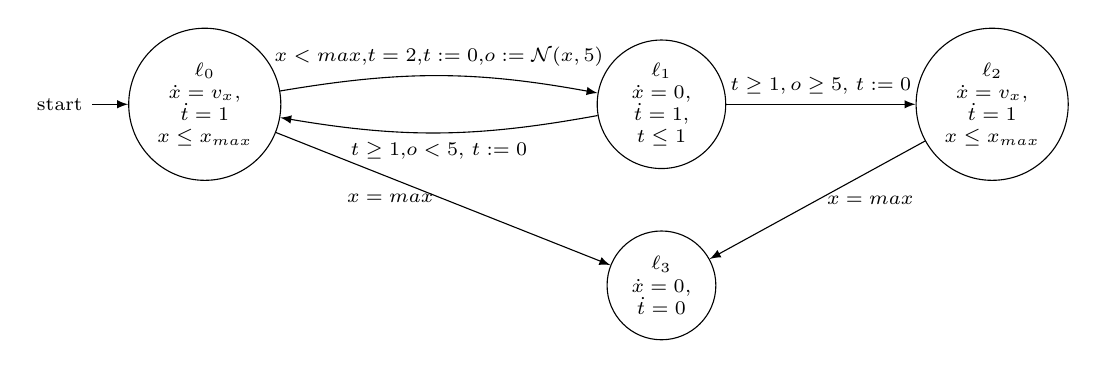
\begin{tikzpicture}[node distance=5cm]%, initial text = {$x,y=0$}]
            \node [state,initial] (s0) {$\ell_{0}$\\$\dot{x}=v_{x},$\\$\dot{t}=1$\\$x\leq x_{max}$};
            \node [state] (s1) [right of = s0,node distance=5.8cm] {$\ell_{1}$\\ $\dot{x}=0,$\\ $\dot{t}=1$,\\ $t\leq1$};
            \node [state] (s2) [right of = s1,node distance=4.2cm] {$\ell_{2}$\\ $\dot{x}=v_{x},$\\ $\dot{t}=1$\\ $x\leq x_{max}$};
            \node [state] (s3) [below of = s1,node distance=2.3cm] {$\ell_{3}$\\ $\dot{x}=0,$\\ $\dot{t}=0$};

            \path[->] (s0) edge [bend left = 10] node [above] {$x<max$,$t=2$,$t:=0$,$o:=\mathcal{N}(x,5)$} (s1)
                    edge node [left] {$x=max$} (s3)
                (s1) edge  [bend left = 10] node [below] {$t\geq 1$,$o< 5$, $t:=0$} (s0)
                    edge node [above] {$t\geq 1, o\geq 5$, $t:=0$} (s2)
                (s2) edge node [right] {$x=max$} (s3);

        \end{tikzpicture}
        \caption{Example of UAV find stochastic hybrid automaton.}
         \label{fig:shauav}
     \end{center}
\end{figure}
We first abstract the continuous distribution functions into discrete distributions. There is only one transition with a continuous distribution in our example (with normal distribution) and the transition lies between location $\ell_{0}$ and $\ell_{1}$. Then for the command abstraction we let $c=(x<max\land t=2\rightarrow \mathcal{N}(x,5):\ell_{1})$. We choose $p_{1}=p_{2}=p_{3}=p_{4}=0.25$. As we have a normal distribution we can use symbolic approximation to find intervals $a_{i}$ which correlate to the probabilities $p_{i}$
\begin{align*}
    a_{1} &\in x+[-3.38,-3.37] \\
    a_{2} &\in x+[-0.1,0.1] \\
    a_{3} &\in x+[3.37,3.38] .
\end{align*}
This approximation changes for different distributions.
From these intervals we can find $\hat{u}_{i}$, for $q=(\ell_{0},x,t,o)$ we know that the reset will be $x:=x$ and $t:=0$.
\begin{align*}
    \hat{u}_{1}(q) & = \{(\ell_{1},x,0)\}\times(-\infty,a_{1}] \\
    \hat{u}_{2}(q) & = \{(\ell_{1},x,0)\}\times(a_{1},a_{2}] \\
    \hat{u}_{3}(q) & = \{(\ell_{1},x,0)\}\times(a_{2},a_{3}] \\
    \hat{u}_{4}(q) & = \{(\ell_{1},x,0)\}\times(a_{3},\infty).
\end{align*}
This sets $L(q)(u_{i}(q))=p_{i}=0.25$ for $i\in\{1,\ldots,4\}$ and $L(q)(\bigcup_{i=1}^{4}\hat{u}_{i}(q))=1$.
Then we can find the $u_{i}$ to be
\begin{align*}
    u_{1}(q) & = \{(\ell_{1},x,0)\}\times(-\infty,-3.37] \\
    u_{2}(q) & = \{(\ell_{1},x,0)\}\times[-3.38,0.1] \\
    u_{3}(q) & = \{(\ell_{1},x,0)\}\times[-0.1,3.38] \\
    u_{4}(q) & = \{(\ell_{1},x,0)\}\times[3.37,\infty) \\
\end{align*}
where $\hat{u}_{i}\subseteq u_{i}$. So we find that the command abstraction is $\mathbf{f}=(\hat{u}_{1},\ldots,\hat{u}_{4},u_{1},\ldots,u_{4},p_{1},\ldots,p_{4})$ and the abstracted guard is
\[
abs(c,\mathbf{f}) = (x<max\land t=2\rightarrow 0.25:u_{1}+\cdots+0.25:u_{4}).
\]

So the PHA that is the abstraction of the SHA in Figure~\ref{fig:shauav} consists of
\begin{itemize}
    \item $V=\{x,t,o\}$
    \item $L=\{\ell_{0},\ell_{1},\ell_{2},\ell_{3}\}$
    \item $\Init=\ell_{0}$
    \item the flow function is
        \begin{align*}
            f(\ell_{0}) &= \{\dot{x}=v_{x},\dot{t}=1,\dot{o}=0\} \\
            f(\ell_{1}) &= \{\dot{x}=0,\dot{t}=1,\dot{o}=0\} \\
            f(\ell_{2}) &= \{\dot{x}=v_{x},\dot{t}=1,\dot{o}=0\} \\
            f(\ell_{3}) &= \{\dot{x}=0,\dot{t}=0,\dot{o}=0\}
        \end{align*}
    \item the discrete transition function $t$ is
        \begin{align*}
            t(\ell_{0}) &= \{x=x_{max}\rightarrow 1:\ell_{3},\ x<max\land t=2\rightarrow 0.25:u_{1}+\cdots+0.25:u_{4}\} \\
            t(\ell_{1}) &= \{o\leq10\rightarrow 1:\ell_{0},\ o>10\rightarrow 1:\ell_{2}\} \\
            t(\ell_{2}) &= \{x=x_{max}\rightarrow 1:\ell_{3}\}.
        \end{align*}
\end{itemize}
Next we need to turn this PHA into a form that we can work with.

%There are two ways this can be approached. T We can reformulate the components to fit the definition of a rectangular PHA and then use the translations discussed in Section~\ref{sec:phatrans} to create a PTA which can be model checked. This rectangular PHA would be defined as
\begin{itemize}
    \item $V=\{x,t,o\}$
    \item $L=\{\ell_{0},\ell_{1,1},\ell_{1,2},\ell_{1,3},\ell_{1,4},\ell_{2},\ell_{3}\}$
    \item $A=\{act_{1},act_{2},act_{3},act_{4},act_{5}\}$, we can choose our action set freely.
    \item $\Init = \{\ell_{0},(\mathbb{R},0,0)\}$
    \item The invariant conditions are
        \begin{align*}
            \Inv(\ell_{0})&=((-\infty,x_{max}],[0,\infty),\mathbb{R}) \\
            \Inv(\ell_{1,1})&=\Inv(\ell_{1,2})=\Inv(\ell_{1,3})=\Inv(\ell_{1,4})=(\mathbb{R},[0,1],\mathbb{R}) \\
            \Inv(\ell_{2})&=((-\infty,x_{max}],[0,\infty),\mathbb{R}) \\
            \Inv(\ell_{3})&=\emptyset
        \end{align*}
    \item The edge set is
    \begin{align*}
        E=\{&e_{1,1}=(\ell_{0},act_{1},\ell_{1,1}),
        e_{1,2}=(\ell_{0},act_{1},\ell_{1,2}), e_{1,3}=(\ell_{0},act_{1},\ell_{1,3}),
        e_{1,4}=(\ell_{0},act_{1},\ell_{1,4}), \\
        & e_{2}=(\ell_{0},act_{2},\ell_{3}), e_{3,1}=(\ell_{1,1},act_{3},\ell_{0}), e_{3,2}=(\ell_{1,2},act_{3},\ell_{0}), e_{3,3}=(\ell_{1,3},act_{3},\ell_{0}), \\
        & e_{3,4}=(\ell_{1,4},act_{3},\ell_{0}), e_{4,1}=(\ell_{1,1},act_{4},\ell_{2}), e_{4,2}=(\ell_{1,2},act_{4},\ell_{2}), e_{4,3}=(\ell_{1,3},act_{4},\ell_{2}), \\
        & e_{4,4}=(\ell_{1,4},act_{4},\ell_{2}), e_{5}=(\ell_{2},act_{5},\ell_{3})\}
    \end{align*}
        with guard conditions
        \begin{align*}
            g(e_{1,1})=&g(e_{1,2})=g(e_{1,3})=g(e_{1,4})=((-\infty,x_{max}),[2,2],\mathbb{R}), \\
            g(e_{2})=&([x_{max},x_{max}],\mathbb{R},\mathbb{R}), \\
            g(e_{3,1})=&g(e_{3,2})=g(e_{3,3})=g(e_{3,4})=(\mathbb{R},[1,\infty),(-\infty,5]), \\
            g(e_{4,1})=&g(e_{4,2})=g(e_{4,4})=g(e_{4,4})=(\mathbb{R},[1,\infty),[5,\infty)), \\
            g(e_{5})=&([x_{max},x_{max}],\mathbb{R},\mathbb{R})
        \end{align*}
        and reset maps
        \begin{align*}
            r(e_{1,1})=&(x,0,(-\infty,-3.37]) \\
            r(e_{1,2})=&(x,0,[-3.38,0.1]) \\
            r(e_{1,3})=&(x,0,[-0.1,3.38]) \\
            r(e_{1,4})=&(x,0,[3.37,\infty)) \\
            r(e_{2})=&(x,t,o) \\
            r(e_{3,1})=&r(e_{3,2})=r(e_{3,3})=r(e_{3,4})=(x,0,o) \\
            r(e_{4,1})=&r(e_{4,2})=r(e_{4,3})=r(e_{4,4})=(x,0,o) \\
            r(e_{5})=&(x,t,o).
        \end{align*}
    \item The flow conditions for each location are
        \begin{align*}
            f(\ell_{0})=&\{\dot{x}=v_{x},\dot{t}=1,\dot{o}=0\} \\
            f(\ell_{1,1})=&f(\ell_{1,2})=f(\ell_{1,3})=f(\ell_{1,4})=\{\dot{x}=0,\dot{t}=1,\dot{o}=0\}\\
            f(\ell_{2})=&\{\dot{x}=v_{x},\dot{t}=1,\dot{o}=0\} \\
            f(\ell_{3})&=\{\dot{x}=0,\dot{t}=0,\dot{o}=0\}.
        \end{align*}
    \item The probabilistic transition function is
        \begin{align*}
            t(\ell_{0},act_{1})=&\{0.25:\ell_{1,1},0.25:\ell_{1,2},0.25:\ell_{1,3},0.25:\ell_{1,4}\} \\
            t(\ell_{0},act_{2})=&\{1:\ell_{3}\} \\
            t(\ell_{1,1},act_{3})=&t(\ell_{1,2},act_{3})=t(\ell_{1,4},act_{3})=t(\ell_{1,4},act_{3})=\{1:\ell_{0}\} \\
            t(\ell_{1,1},act_{4})=&t(\ell_{1,2},act_{4})=t(\ell_{1,4},act_{4})=t(\ell_{1,4},act_{4})=\{1:\ell_{2}\} \\
            t(\ell_{2},act_{5})=&\{1:\ell_{3}\}.
        \end{align*}
\end{itemize}
The above automaton is clearly a rectangular probabilistic hybrid automaton, which we can translate into a PTA.
% Instead we will use the abstraction technique described earlier in this section in Definition~\ref{def:phs2lts}.
% We choose the abstract state space to be
% \begin{align*}
% Q_{A}=\{&(\ell_{0},(-\infty,x_{max}),(-\infty,2],\mathbb{R}), (\ell_{0},[x_{max},\infty),(2,\infty),\mathbb{R}), (\ell_{1},\mathbb{R},(-\infty,1],(-\infty,-3.37]), \\
% & (\ell_{1},\mathbb{R},(-\infty,1],[-3.38,0.1]), (\ell_{1},\mathbb{R},(-\infty,1],[-0.1,3.38]), (\ell_{1},\mathbb{R},(-\infty,1],[3.37,\infty)) \\
% & (\ell_{1},\mathbb{R},(1,\infty),(-\infty,-3.37]), (\ell_{1},\mathbb{R},(1,\infty),[-3.38,0.1]), (\ell_{1},\mathbb{R},(1,\infty),[-0.1,3.38]), \\
% & (\ell_{1},\mathbb{R},(1,\infty),[3.37,\infty)), (\ell_{2},(-\infty,x_{max}),\mathbb{R},\mathbb{R}), (\ell_{2},[x_{max},\infty),\mathbb{R},\mathbb{R}), \\
% & (\ell_{3},\mathbb{R},\mathbb{R},\mathbb{R})
% \}
% \end{align*}
% by using the the invariance and guard conditions of the locations. Similarly we define the time restrictions to be $\mathbf{T}=\{\mathbf{t}_{\ell{0}},\mathbf{t}_{\ell{1}},\mathbf{t}_{\ell{2}},\mathbf{t}_{\ell{3}}\}$
% \begin{align*}
%     \mathbf{t}_{\ell{0}}=& \frac{x_{max}}{v_{x}}\\
%     \mathbf{t}_{\ell{1}}=& 1\\
%     \mathbf{t}_{\ell{2}}=& \frac{x_{max}}{v_{x}}\\
%     \mathbf{t}_{\ell{3}}=& 10.
% \end{align*}
% based on the continuous behaviour of the variables, the guard and invariance conditions. As there is no continuous flow in $\ell_{3}$ we set an arbitrary time out.
%
% With $Q_{A}$ and $\mathbb{T}$ we can now find the LTS abstraction of our PHA, to be
% \begin{itemize}
%     \item $Q=Q_{A}$
%     \item $Q_{0}=\{(\ell_{0},0,0,0)\}$
%     \item $A=\{t(\ell_{0}),t(\ell_{1}),t(\ell_{2}),\bot\}$
%     \item
% \end{itemize}
\end{ex}


\subsection{Abstracting Discrete Time Stochastic Hybrid Systems}
In this section we will show how to abstract a DTSHS $\mathcal{D}=(L,n,\Init,T_x,T_q,R)$ to a discrete time markov chain, which then can be model checked using the usual techniques.

Before we get to the abstraction we give a couple preliminary definitions and notations.

\begin{defi}[Partition of the State Space]
Let $\mathcal{Q}=\bigcup_{\ell\in L}\{\ell\} \times Q_{\ell}$ be the state space, where $Q_{\ell}\subset \mathbb{R}^{n(\ell)}$ (see the Definition~\ref{def:DTSHS} for $n$) is a compact
set, with $Q_{\ell} = \bigcup_{i=1}^{m_{\ell}} Q_{\ell,i}$ having a finite partition and $Q_{\ell,i}\in \mathcal{B}(\mathbb{R}^{n(\ell)})$ $Q_{\ell,i}\cap Q_{\ell,j} = \emptyset$ for all
$i\neq j$, $m_{\ell}\in\mathbb{N}$ is number of partitions of the continous domain of $\ell$.
\end{defi}

\begin{defi}[Partition Representative]
We define $r_{\ell}:\mathcal{B}(\mathbb{R}^{n(\ell)})\rightarrow\mathbb{R}^{n(\ell)}$ to be the function returning the \emph{representative point} $r_{\ell}(Q_{\ell,i})$ of the partition $Q_{\ell,i}$, which is a randomly chosen point given
 $Q_{\ell,i}\in\mathcal{B}(\mathbb{R}^{n(\ell)})$ and $\ell\in L$.
\end{defi}


\begin{defi}[DTSHS to DTMC Abstraction \cite{Abate2010,Abate2011}]
Let $\mathcal{D}=(L,n,\Init,T_x,T_q,R)$ be a DTSHS. Then the DTMC associated to $\mathcal{D}$ $\mathcal{C}=(\mathcal{Q}_{\delta},\Init_{\delta},t_{\delta})$ is defined as
\begin{itemize}
    \item $\mathcal{Q}_{\delta}=\{(\ell,i) : \ell \in L, i\in\{1,\ldots,m_{\ell}\}\}$ is the state space, $m_{\ell}\in \mathbb{N}$;
    \item $\Init_{\delta}(\ell,i) = \int_{Q_{\ell,i}} \Init(\ell,x) dx$ is the probability distribution for the initial state;
    \item $t_{\delta}((\ell,i),(\ell',i')) = T(\ell'\times Q_{\ell',i'}, (\ell,r_{\ell}(Q_{\ell,i})))$ is the transition probability matrix.
\end{itemize}
\end{defi}

%\begin{defi}[Gridding]
%Let $\delta_{\ell,i} = \sup\{ \| x-x'\| : x,x'\in Q_{\ell,i}\}$ be the \emph{diameter} of $Q_{\ell,i}$. We also define $\delta=\max_{i\in\{1,\ldots,m_{\ell},\ell\in L} \delta_{\ell,i}$ to be the \emph{grid size parameter},
%\end{defi}


%\cite{Abate2010,Amin2006,Hahn2011,Hofbaur2002,Julius2009,Kattenbelt2009,Soudjani2011a,Bujorianu2004,Koutsoukos2006,Hu2000,Prandini2006}

%\cite{Hahn2011} uses game-theory to produce the abstraction and an optimal choice.

%\cite{Kattenbelt2009} uses a mix of predicate and CEGAR.



\subsection{Counterexample-guided abstraction refinement (CEGAR)}
\label{sec:cegar}
\input{cegar}


%\subsection{Flowpipe approximation}
%Type of approximation of the reachable set of states.

\subsection{Barrier certificates}
\label{sec:barrier}
\input{barrier}
%Used to determine upper bound of reachability of sets of states.

\subsection{Phase Portrait Approximation}
\label{sec:phase}
Abstraction goes from HA to rectangular HA.
\cite{Henzinger1998,Raskin2005}

\cite{Henzinger1998} has a two step abstraction, first clock transition then PP

\cite{Raskin2005} has citations


\subsection{Other Abstractions}
\label{sec:misc}
\cite{Fecher2006} going from MC to AMC, but introducing three valued truths, such that when going up we can determine what is definitely true, and definitely false.

\cite{Halbwachs1994} convex approximation of reachability used to make HS more verifiable.

\cite{Henzinger} convex approximation used in HyTech



\subsection{Some known hybrid automata which are undecidable}
\label{sec:undec}
\begin{thm}[\cite{Henzinger1995}]
Consider the class of linear hybrid automata with $n-1$ continuous variables, where all $x$ have derivative $f(\ell)=\dot{x}=1$, $\forall\ell\in L$, and one two slope variable with slopes $k_{1}\neq k_{2}$, which means that $f(\ell,x)=k_{1}$ or $f(\ell,x)=k_{2}$ $\forall\ell\in L$. Then the reachability problem \ref{prob:reach} is undecidable.
\end{thm}

\begin{thm}[\cite{Henzinger1995}]
Suppose we generalize the definition of linear hybrid automata so to permit
\begin{enumerate}
    \item{the intersection of rectangular guard sets $g(e)$ with inequalities of the form $x_{i}\leq x_{j}$,}
    \item{the intersection of rectangular invariant sets $Inv(\ell)$ with inequalities of the form $x_{i}\leq x_{j}$,}
    \item{reset maps $r(e)$ of the form $x_{i}=x_{j}$, for $j\neq i$.}
\end{enumerate}
Consider a class of linear hybrid automata that are generalized in one of these three ways and that have $n-1$ continuous variables of the form $\dot{x}=1$ and a one-slope variable with slope $k\neq1$. The reachability problem \ref{prob:reach} is undecidable for this class of hybrid automata.
\end{thm}

\begin{thm}[\cite{Henzinger2000}]
The reachability problem (Problem~\ref{prop:reach}) for multi-singular automata and for triangular automata are undecidable.
\end{thm}



\begin{table}
\begin{center}
\begin{tabular}{|l|l|l|l|l|l|l|l|l|}\hline
Type & Discrete & Predicate & Bisimulation & $\mu$ & Probabilistic & CEGAR & Barrier & Phase Portrait \\ \hline
Rectangular &  &  &  &  &  &  &  & \\ \hline
Linear &  &  &  &  &  &  &  & \\ \hline
Timed &  &  &  &  &  &  &  & \\ \hline
Stochastic &  &  &  &  &  &  &  & \\ \hline
O-Minimal &  &  &  &  &  &  &  & \\ \hline
\end{tabular}
\label{tab:abssummary}
\caption{Summary of the presented types of hybrid systems.}
\end{center}
\end{table}



\section{Tools}
\label{sec:tools}
\cite{Silva2001} is a survey over some tools.

\cite{Raskin2005} contains citations for CHARON and d/dt.

\begin{itemize}
    \item{KeYmaera \cite{Platzer2011a}}
    \item{KRONOS \cite{Nicollin1993,Alur1997}}
    \item{UPAAL \cite{Alur1997}}
    \item{HyTech \cite{Henzinger1997,Alur1997,Alur1996,Henzinger}}
    \item{SAL \cite{Tiwari2002}}
    \item{CHARON}
    \item{$d/dt$ \cite{Asarin2002,Asarin2000}}
    \item{STEP \cite{}}
    \item{CHECKMATE}
    \item{PHAVer}
    \item{SMV}
    \item{VIS}
    \item{HySAT}
    \item{level-set method}
    \item{COSPAN}
\end{itemize}


%\nocite*
\bibliographystyle{amsplain}
%\bibliography{../../Desktop/PhD/Papers/Bibliography/library}
%\bibliography{library}
\bibliography{copylibrary}

\end{document}
